\subsection{Sequencer}
\subsubsection{Overview}

The Sequencer is a critical off-chain component of the ZK-Rollup responsible for collecting, validating, ordering, and batching user transactions before they are processed by the Executor. Implemented in Rust for performance and memory safety, the Sequencer acts as the primary interface between end-users and the rollup's execution layer, while also maintaining synchronization with Layer 1 (L1) Ethereum to handle priority operations. By handling the complexity of transaction ordering and validation off-chain, the Sequencer enables the high throughput and low latency characteristic of rollups, deferring the computationally expensive proof generation to the Executor.

\subsubsection{Architectural Components}

\begin{figure}[htbp]
 \begin{adjustwidth}{0cm}{}
  \centering
  \includegraphics[height=0.95\linewidth, angle=0]{figures/sequencer.png}
  \caption{Sequencer architecture.}
  \label{fig:operation-flow}
 \end{adjustwidth}
\end{figure}

The sequencer is implemented as a modular Rust crate, organized into clearly separated components. Several well-known design patterns---including Strategy, Factory Method, Composition Root, Shared State, Observer, and Pipeline---are applied throughout the implementation to achieve extensibility and maintainability. Each pattern is discussed in context within the component that employs it.

\subsubsubsection{Sequencer API (JSON-RPC Endpoint)}

The Sequencer API serves as the public gateway for all user interactions with the rollup. By exposing a JSON-RPC interface compatible with standard Ethereum wallet clients, it allows users to submit signed transactions using familiar tooling (e.g., MetaMask, ethers.js) without needing specialized software.

The application startup follows the \textbf{Composition Root} pattern: the \texttt{main.rs} entry point creates all shared resources (state cache, transaction pools) at the top level and distributes them to components via \texttt{Arc} references, wiring three concurrent async tasks---the API server, the L1 listener, and the batch orchestrator:

\begin{lstlisting}[style=rustStyle, caption={Composition root wiring components}, label={lst:main}]
let state_cache = StateCache::new();
let tx_pool = Arc::new(TransactionPool::new());
let forced_queue = Arc::new(ForcedQueue::new());

// L1 listener and batch orchestrator run as background tasks
tokio::spawn(async move { l1_listener.start().await; });
tokio::spawn(async move { orchestrator.start().await; });

// API server blocks on main thread
server.start().await
\end{lstlisting}

The API itself is implemented using the \textbf{Axum} web framework with Tokio as the async runtime. Incoming JSON-RPC requests are routed to handlers based on the method name. The \texttt{sendTransaction} handler orchestrates the full transaction lifecycle---deserialization, validation, pool insertion, and soft confirmation:

\begin{lstlisting}[style=rustStyle, caption={Transaction submission handler}, label={lst:send-tx}]
async fn handle_send_transaction(state: AppState, request: JsonRpcRequest)
    -> Json<JsonRpcResponse>
{
    let tx: UserTransaction = serde_json::from_value(request.params.clone())?;
    match state.validator.validate(&tx).await {
        Ok(()) => {
            state.state_cache.increment_nonce(&tx.from).await;
            state.tx_pool.add(tx.clone()).await;
            // Return SoftConfirmation with Accepted status
        }
        Err(validation_error) => {
            // Return SoftConfirmation with Rejected { reason } status
        }
    }
}
\end{lstlisting}

\subsubsubsection{Validity Checker}

Before entering the transaction pool, all submitted transactions must pass through a rigorous multi-stage validation pipeline to ensure network integrity and prevent spam. The \texttt{Validator} performs three sequential checks against the state cache:

\begin{lstlisting}[style=rustStyle, caption={Three-stage validation pipeline}, label={lst:validator}]
pub async fn validate(&self, tx: &UserTransaction)
    -> Result<(), ValidationError>
{
    self.verify_signature(tx)?;    // ECDSA signature recovery
    self.check_nonce(tx).await?;   // Sequential nonce enforcement
    self.check_balance(tx).await?; // Sufficient funds for value + gas
    Ok(())
}
\end{lstlisting}

\paragraph{Signature Verification}
The checker uses ECDSA signature recovery to verify that the transaction was signed by the claimed sender. The recovered address is compared against the \texttt{from} field---a mismatch indicates forgery.

\paragraph{Nonce Validation}
Each transaction's nonce must exactly match the account's current nonce, enforcing strict sequential ordering and preventing replay attacks.

\paragraph{Balance Verification}
The checker confirms the sender has sufficient funds to cover both the transfer value and gas fees (\texttt{gas\_price} $\times$ \texttt{gas\_limit}), filtering out invalid transactions early.

\subsubsubsection{Local State Cache}

To achieve high throughput, the Sequencer relies on the Local State Cache, an in-memory key-value store that maintains a fast-access replica of the current rollup state. The cache applies the \textbf{Shared State} pattern: it is implemented using a \texttt{HashMap<Address, AccountState>} protected by Tokio's asynchronous \texttt{RwLock} and wrapped in \texttt{Arc}, enabling concurrent read access during validation with exclusive writes for nonce updates. This same pattern is applied to the transaction pool and forced queue, allowing all concurrent components to safely share data.

A key design choice is the \texttt{get\_or\_init\_account} method, which returns default values (zero balance, nonce 0) for unknown accounts \emph{without} inserting them into the cache, preventing memory inflation from validation attempts against non-existent accounts.

This cache is periodically synchronized with updates from the State Manager component in the Executor, implementing an eventually-consistent model that accepts brief staleness in exchange for sub-millisecond read latencies during validation.

\subsubsubsection{Transaction Pool}

Valid normal (non-priority) transactions are held in the Transaction Pool, implemented as a FIFO queue using Rust's \texttt{VecDeque} for efficient $O(1)$ insertion and removal. The \texttt{get\_pending(max)} method atomically drains up to \texttt{max} transactions, ensuring each transaction is consumed exactly once by the batch production pipeline.

\subsubsubsection{L1 Event Listener}

The L1 Event Listener follows the \textbf{Observer} pattern: it subscribes to blockchain events from the RollupBridge smart contract on Ethereum L1 and reacts to deposit and forced-exit notifications by populating the forced transaction queue. It uses the \texttt{ethers-rs} library's \texttt{abigen!} macro to create type-safe event filters directly from Solidity event signatures, and connects via WebSocket for real-time event streaming.

The listener uses Tokio's \texttt{select!} macro to concurrently process both Deposit and ForcedExit event streams. Each detected event is parsed into a \texttt{ForcedTransaction} and added to the forced queue. The listener implements an automatic reconnection loop with block checkpoint tracking, maintaining an at-least-once delivery guarantee---if the WebSocket connection drops, it resumes from the last processed block after a configurable retry delay.

\subsubsubsection{Forced Transaction Queue}

Forced transactions originating from L1 events are placed in a dedicated priority queue, separate from the normal transaction pool. This design enforces a critical security property: \textbf{forced transactions are unskippable}. The \texttt{get\_all()} method atomically drains the entire queue, and the batch orchestrator must include all returned transactions in the next batch, preventing censorship and ensuring users can always exit the rollup even if the sequencer becomes malicious or unresponsive.

The forced queue implements strict FIFO ordering based on the order in which L1 events are received (corresponding to L1 block number and transaction index), ensuring deterministic processing order that can be verified by anyone monitoring the L1 chain.

\subsubsubsection{Scheduler (Policy Engine)}
\label{sec:scheduler}

The Scheduler implements the \textbf{Strategy design pattern} \cite{gamma1994design}, allowing the transaction ordering algorithm to be selected at runtime through configuration. The pattern decouples the scheduling context from the concrete ordering implementations through a trait interface:

\begin{figure}[htbp]
\centering
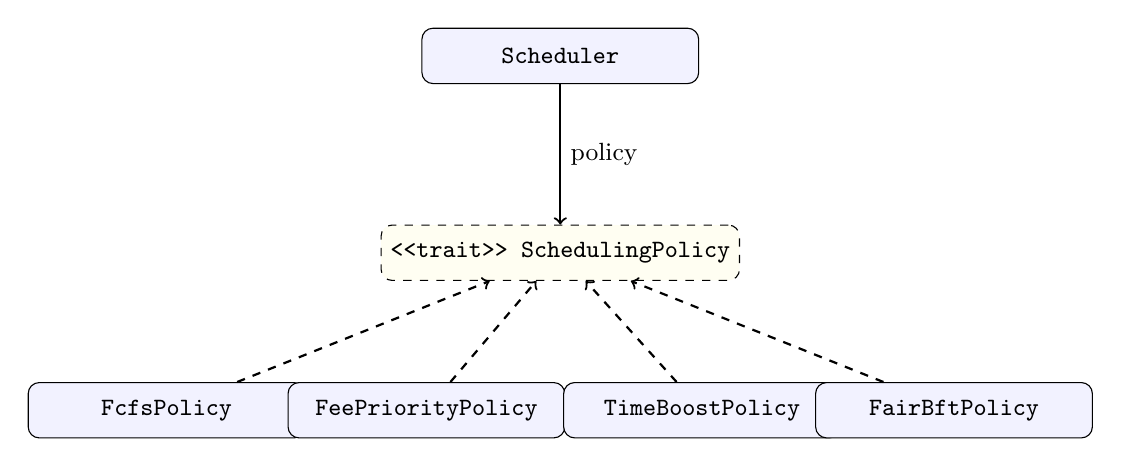
\begin{tikzpicture}[
    class/.style={rectangle, draw=black, rounded corners, minimum height=2em, minimum width=10em, font=\ttfamily\small, fill=blue!5},
    interface/.style={rectangle, draw=black, rounded corners, dashed, minimum height=2em, minimum width=10em, font=\ttfamily\small, fill=yellow!5},
    arrow/.style={->, thick},
    impl/.style={->, thick, dashed},
]
    % Interface
    \node[interface] (trait) at (0, 0) {<<trait>> SchedulingPolicy};
    
    % Context
    \node[class] (scheduler) at (0, 2.5) {Scheduler};
    
    % Concrete strategies
    \node[class] (fcfs) at (-5, -2) {FcfsPolicy};
    \node[class] (fee) at (-1.7, -2) {FeePriorityPolicy};
    \node[class] (tb) at (1.8, -2) {TimeBoostPolicy};
    \node[class] (bft) at (5, -2) {FairBftPolicy};
    
    % Relationships
    \draw[arrow] (scheduler) -- node[right, font=\small] {policy} (trait);
    \draw[impl] (fcfs) -- (trait);
    \draw[impl] (fee) -- (trait);
    \draw[impl] (tb) -- (trait);
    \draw[impl] (bft) -- (trait);
\end{tikzpicture}
\caption{Strategy design pattern applied to scheduling policies.}
\label{fig:strategy-pattern}
\end{figure}

The \texttt{SchedulingPolicy} trait defines the contract that all ordering strategies must implement. The \texttt{Scheduler} holds a boxed trait object (\texttt{Box<dyn SchedulingPolicy>}) for runtime polymorphism, and its \texttt{schedule()} method implements a two-phase ordering algorithm:

\begin{lstlisting}[style=rustStyle, caption={Strategy trait and scheduler context}, label={lst:scheduler}]
// Strategy interface
pub trait SchedulingPolicy: Send + Sync {
    fn order_transactions(&self, txs: Vec<UserTransaction>)
        -> Vec<UserTransaction>;
    fn name(&self) -> &str;
}

// Context: holds a strategy and applies two-phase ordering
pub struct Scheduler {
    policy: Box<dyn SchedulingPolicy>,  // Runtime-selected strategy
}

impl Scheduler {
    pub fn schedule(&self, forced: Vec<ForcedTransaction>,
                    normal: Vec<UserTransaction>) -> Vec<Transaction> {
        let mut result = Vec::new();
        // Phase 1: ALL forced transactions first (non-negotiable)
        for tx in forced { result.push(Transaction::Forced(tx)); }
        // Phase 2: Normal transactions ordered by selected policy
        for tx in self.policy.order_transactions(normal) {
            result.push(Transaction::Normal(tx));
        }
        result
    }
}
\end{lstlisting}

The scheduling policy is selected through the TOML configuration file, parsed into a \texttt{SchedulingPolicyType} enum, and instantiated via a \textbf{Factory Method} pattern. The \texttt{create\_policy()} function maps each enum variant to its concrete policy implementation, decoupling policy creation from usage:

\begin{lstlisting}[style=rustStyle, caption={Factory method for policy creation}, label={lst:factory}]
pub fn create_policy(policy_type: SchedulingPolicyType)
    -> Box<dyn SchedulingPolicy>
{
    match policy_type {
        SchedulingPolicyType::Fcfs => Box::new(FcfsPolicy),
        SchedulingPolicyType::FeePriority => Box::new(FeePriorityPolicy),
        SchedulingPolicyType::TimeBoost { time_window_ms } =>
            Box::new(TimeBoostPolicy { time_window_ms }),
        SchedulingPolicyType::FairBft => Box::new(FairBftPolicy),
    }
}
\end{lstlisting}

This enables runtime switching without code changes:

\begin{lstlisting}[language={}, caption={Switching scheduling policy via configuration}, label={lst:sched-config}]
[scheduling]
policy_type = "FCFS"        # Options: "FCFS", "FeePriority",
                            #          "TimeBoost", "FairBFT"
time_window_ms = 5000       # Only used for TimeBoost policy
\end{lstlisting}

Four concrete strategies are implemented, each encapsulating a distinct ordering algorithm:

\begin{itemize}
    \item \textbf{FCFS (First-Come-First-Served)}: Maintains the original submission order with $O(1)$ overhead---the simplest and most predictable policy.
    \item \textbf{Fee-Priority}: Sorts transactions by \texttt{gas\_price} in descending order ($O(n \log n)$), maximizing sequencer revenue but potentially starving low-fee transactions.
    \item \textbf{Time-Boost}: Divides time into configurable discrete windows (e.g., 5-second slots) and applies a multi-key sort within each window---first by \texttt{boost\_bid} (a premium bid field), then by \texttt{gas\_price}, then FCFS for tie-breaking. This provides predictable latency guarantees with granular fairness.
    \item \textbf{Fair BFT Ordering}: Sorts strictly by transaction timestamp (ascending) to provide time-based fairness and MEV resistance. The current implementation targets a single-node sequencer; a multi-node extension would add BFT consensus for canonical timestamp agreement.
\end{itemize}

As an example, the Fee-Priority strategy simply sorts by gas price, while the Time-Boost strategy uses a more complex multi-key comparator:

\begin{lstlisting}[style=rustStyle, caption={Concrete strategy implementations (Fee-Priority and Time-Boost)}, label={lst:policies}]
// Fee-Priority: highest gas price first
impl SchedulingPolicy for FeePriorityPolicy {
    fn order_transactions(&self, mut txs: Vec<UserTransaction>)
        -> Vec<UserTransaction> {
        txs.sort_by(|a, b| b.gas_price.cmp(&a.gas_price));
        txs
    }
}

// Time-Boost: windowed ordering with premium bids
impl SchedulingPolicy for TimeBoostPolicy {
    fn order_transactions(&self, mut txs: Vec<UserTransaction>)
        -> Vec<UserTransaction> {
        txs.sort_by(|a, b| {
            let window_a = a.timestamp / self.time_window_ms;
            let window_b = b.timestamp / self.time_window_ms;
            match window_a.cmp(&window_b) {
                Ordering::Equal => {
                    let boost_a = a.boost_bid.unwrap_or_default();
                    let boost_b = b.boost_bid.unwrap_or_default();
                    match boost_b.cmp(&boost_a) {
                        Ordering::Equal => b.gas_price.cmp(&a.gas_price),
                        other => other,
                    }
                }
                other => other,
            }
        });
        txs
    }
}
\end{lstlisting}

This Strategy-based architecture satisfies the Open/Closed Principle: new ordering policies can be added by implementing the \texttt{SchedulingPolicy} trait without modifying the existing scheduler or orchestrator code, and different policies can be benchmarked under identical workloads by changing a single configuration value.

\subsubsubsection{Batch Engine}

The Batch Engine aggregates ordered transactions into sealed batches ready for execution. It maintains a monotonically increasing batch ID counter and enforces gas limits by tracking cumulative gas consumption as transactions are added:

\begin{lstlisting}[style=rustStyle, caption={Gas limit enforcement in batch engine}, label={lst:gas-limit}]
pub fn can_add_transaction(&self, current_txs: &[Transaction],
                            new_tx: &Transaction) -> bool {
    let current_gas: u64 = current_txs.iter()
        .map(|tx| tx.gas_limit()).sum();
    let total_gas = current_gas.saturating_add(new_tx.gas_limit());
    total_gas <= self.config.max_gas_limit
}
\end{lstlisting}

This check ensures no batch exceeds the configured gas limit that would make L1 verification prohibitively expensive. The \texttt{saturating\_add} prevents integer overflow during gas accumulation.

\subsubsubsection{Batch Orchestrator}

The Batch Orchestrator implements the \textbf{Pipeline} pattern, coordinating a multi-stage batch production flow: transactions move from Queue $\rightarrow$ Scheduler $\rightarrow$ BatchEngine $\rightarrow$ sealed Batch. It connects the forced queue, transaction pool, scheduler, and batch engine, running as a background async task with a dual-trigger batching mechanism:

\paragraph{Time-Based Trigger}
If the configured \texttt{timeout\_interval\_ms} expires before reaching the size threshold, the engine seals a partial batch to prevent unbounded latency during low-activity periods.

\paragraph{Size-Based Trigger}
When the number of queued transactions reaches the configured \texttt{max\_batch\_size}, a batch is immediately sealed.

The core \texttt{produce\_batch} method implements a four-step pipeline: (1) drain all forced transactions from the L1 queue, filtering by gas limit; (2) pull normal transactions from the pool, enforcing both size and gas limits; (3) combine both sets with forced transactions first; and (4) seal the batch via the \texttt{BatchEngine}.

\subsubsubsection{Batch Configuration}
\label{sec:batch-config}

The Sequencer's behavior is driven by a TOML configuration file loaded through Rust's \texttt{serde} deserialization framework. The configuration is organized into five sections, each mapping to a dedicated Rust struct:

\begin{lstlisting}[style=rustStyle, caption={Configuration structure hierarchy}, label={lst:config-structs}]
#[derive(Debug, Clone, Deserialize)]
pub struct Config {
    pub batch: BatchConfig,         // Batching parameters
    pub scheduling: SchedulingConfig, // Policy selection
    pub api: ApiConfig,             // JSON-RPC endpoint
    pub l1: L1Config,               // L1 connection settings
    pub database: DatabaseConfig,   // Registry storage
}
\end{lstlisting}

At startup, the configuration is loaded from a TOML file and used to initialize all components. The configuration flow works as follows: the \texttt{Config::load()} method reads and parses the TOML file, then each section is passed to its corresponding component. For example, the scheduling policy is resolved from the string-based TOML value (\texttt{"FCFS"}, \texttt{"FeePriority"}, etc.) into a \texttt{SchedulingPolicyType} enum, which the factory function (Listing~\ref{lst:factory}) uses to instantiate the correct strategy object:

\begin{lstlisting}[style=rustStyle, caption={Configuration to component wiring}, label={lst:config-wiring}]
let config = Config::load("config/default.toml")?;

// Scheduling policy: TOML string -> enum -> concrete strategy
let orchestrator = BatchOrchestrator::new(
    forced_queue.clone(),
    tx_pool.clone(),
    config.batch.clone(),                // BatchConfig -> engine
    config.scheduling.to_policy_type(),  // "FCFS" -> SchedulingPolicyType::Fcfs
);
\end{lstlisting}

The batch-specific parameters directly control the throughput-latency-cost trade-off. The default configuration demonstrates the tunable parameters:

\begin{lstlisting}[language={}, caption={Default sequencer configuration (\texttt{config/default.toml})}, label={lst:default-config}]
[batch]
max_batch_size = 100          # Max transactions per batch
timeout_interval_ms = 5000    # Seal partial batch after 5 seconds
min_batch_size = 10           # Minimum transactions before timeout seal
max_gas_limit = 30000000      # 30M gas limit per batch

[scheduling]
policy_type = "FCFS"          # Transaction ordering strategy

[api]
host = "127.0.0.1"
port = 3000

[l1]
rpc_url = "https://sepolia.infura.io/v3/YOUR_KEY"
bridge_address = "0x742d35Cc6634C0532925a3b844Bc9e7595f0bEb"
start_block = 18500000

[database]
url = "sqlite://sequencer.db"
\end{lstlisting}

These parameters directly influence system behavior:
\begin{itemize}
    \item \textbf{max\_batch\_size} and \textbf{timeout\_interval\_ms}: Larger batches and longer timeouts amortize fixed costs (proof generation, L1 submission) across more transactions, reducing per-transaction cost but increasing user-perceived latency. Smaller values improve responsiveness at the expense of higher overhead.
    \item \textbf{max\_gas\_limit}: Caps the computational cost per batch to ensure L1 proof verification remains economical. The batch engine uses the \texttt{can\_add\_transaction()} method (Listing~\ref{lst:gas-limit}) to enforce this limit iteratively as transactions are added.
    \item \textbf{policy\_type}: Selects the scheduling strategy at runtime (see Section~\ref{sec:scheduler}), enabling experimental comparison without recompilation.
\end{itemize}

The optimal configuration depends on network activity patterns and application requirements, which is why these parameters are exposed for experimental tuning in this research prototype.

\subsubsubsection{Batch Registry}

The Batch Registry is a persistent metadata store (backed by SQLite via the \texttt{sqlx} crate) that records the history of all produced batches. For each batch, it stores lightweight metadata: batch ID, transaction counts (total and forced), creation timestamp, and the scheduling policy used. This registry serves as an audit trail for verifiable sequencer decisions, enables crash recovery after restarts, and supports post-hoc analysis of batching efficiency and policy effectiveness during benchmarking.

\subsubsection{Operational Flow}

\begin{figure}[htbp]
 \begin{adjustwidth}{0cm}{}
  \centering
  \includegraphics[height=0.95\linewidth, angle=0]{figures/sequencer_pipeline.png}
  \caption{Sequencer flow.}
  \label{fig:sequencer-pipeline-flow}
 \end{adjustwidth}
\end{figure}

The complete sequencer workflow proceeds as follows:

\begin{enumerate}
    \item \textbf{User Transaction Submission}: A user submits a signed \texttt{UserTransaction} to the Sequencer API JSON-RPC endpoint via an HTTP POST request.
    
    \item \textbf{Validation}: The \texttt{Validator} performs three sequential checks against the \texttt{StateCache}: ECDSA signature verification, nonce validation, and balance sufficiency. Valid transactions receive a \texttt{SoftConfirmation} with \texttt{Accepted} status; invalid transactions are rejected immediately with a descriptive \texttt{ValidationError}.
    
    \item \textbf{Pool Insertion}: Valid transactions are inserted into the \texttt{TransactionPool} (FIFO queue), awaiting batch inclusion. The sender's nonce is immediately incremented in the \texttt{StateCache}.
    
    \item \textbf{L1 Event Monitoring}: Concurrently, the \texttt{L1Listener} streams \texttt{Deposit} and \texttt{ForcedExit} events from the RollupBridge contract via WebSocket and places corresponding \texttt{ForcedTransaction} instances into the \texttt{ForcedQueue}.
    
    \item \textbf{Scheduling}: When the \texttt{BatchOrchestrator} timer fires (controlled by \texttt{timeout\_interval\_ms}), the orchestrator pulls transactions from both queues and the \texttt{Scheduler} combines them:
    \begin{itemize}
        \item All pending forced transactions first (FIFO by L1 arrival order)
        \item Normal transactions ordered by the selected \texttt{SchedulingPolicy} (FCFS, FeePriority, TimeBoost, or FairBFT)
    \end{itemize}
    
    \item \textbf{Gas Limit Enforcement}: The orchestrator iteratively checks each transaction against the cumulative gas limit using \texttt{BatchEngine::can\_add\_transaction()}, stopping when the configured \texttt{max\_gas\_limit} is reached.
    
    \item \textbf{Batch Sealing}: The \texttt{BatchEngine} bundles the ordered transaction sequence, assigns a sequential Batch ID, records a UTC timestamp, and produces a sealed \texttt{Batch} ready for forwarding to the Executor component.
\end{enumerate}

\subsubsection{Design Rationale and Trade-offs}

\paragraph{Dual-Queue Architecture}

The separation of forced and normal transaction queues is a deliberate security design. By making forced transactions unskippable and always-first, the sequencer cannot censor user withdrawals even under malicious operation. This property is essential for maintaining the ``escape hatch'' that allows users to exit to L1 if the L2 becomes untrustworthy.

\paragraph{Configurable Scheduling Policies (Strategy Pattern)}

Different use cases demand different ordering guarantees. Financial applications may prioritize fee-based ordering to incentivize faster settlement, while gaming or social applications may prefer FCFS fairness. By applying the Strategy design pattern with a \texttt{SchedulingPolicy} trait and \texttt{Box<dyn SchedulingPolicy>} dynamic dispatch, the sequencer enables:

\begin{itemize}
    \item \textbf{Runtime configuration}: Switching policies via TOML without recompilation
    \item \textbf{Open/Closed Principle}: New policies are added by implementing the trait, without modifying existing code
    \item \textbf{Empirical comparison}: Different ordering rules can be benchmarked under identical workloads
\end{itemize}

\paragraph{Local State Cache vs. Authoritative State}

The Local State Cache trades strict consistency for performance. The \texttt{Arc<RwLock<HashMap>{>}{>}} design allows multiple concurrent readers (validation checks) with exclusive writers (nonce updates), enabling sub-millisecond read latencies. The cache accepts the risk of occasionally admitting transactions that will fail during execution (e.g., due to concurrent balance changes), relying on the Executor to enforce final correctness.

\paragraph{Async Concurrency Model}

The sequencer leverages Tokio's async runtime to run three concurrent components---the API server, L1 listener, and batch orchestrator---on a shared thread pool. Shared state is accessed through \texttt{Arc<RwLock<T>{>}{>}} wrappers, maximizing throughput on modern multi-core hardware without the overhead of inter-process communication.

\paragraph{Batch Size and Timeout Trade-offs}

The dual-trigger batching mechanism balances efficiency and responsiveness. The optimal configuration depends on network activity patterns and application requirements, which is why these parameters are exposed as TOML configuration for experimental tuning (see Section~\ref{sec:batch-config}).

\subsubsection{Integration with Other Components}

The Sequencer interfaces with:

\begin{itemize}
    \item \textbf{RollupBridge Contract (L1)}: Receives deposit and forced-exit events via WebSocket subscription using the \texttt{ethers-rs} library, generating priority forced transactions
    \item \textbf{Executor}: Forwards sealed \texttt{Batch} objects for state transition computation and proof generation
    \item \textbf{State Manager}: Receives state updates to keep the \texttt{StateCache} synchronized via the \texttt{update()} method
    \item \textbf{Users}: Provides the JSON-RPC API (via Axum) for transaction submission and soft confirmation responses
\end{itemize}

This modular design isolates sequencing logic from execution and proving, enabling independent optimization and replacement of components during benchmarking experiments.


This sequencer component forms the critical first stage of the ZK-Rollup pipeline, transforming a stream of user requests and L1 events into ordered, validated batches ready for cryptographic proof generation---bridging the gap between user experience and the mathematical guarantees provided by zero-knowledge proofs.



\subsection{Executor}
\subsubsection{Overview}
The executor constitutes a high-performance zkRollup execution engine implemented in Rust, designed to process Ethereum-compatible transaction batches as the computational backbone of a Layer-2 scaling solution. The architectural philosophy centers on separation of concerns and modular composability. 

\begin{figure}[H]
    \centering
    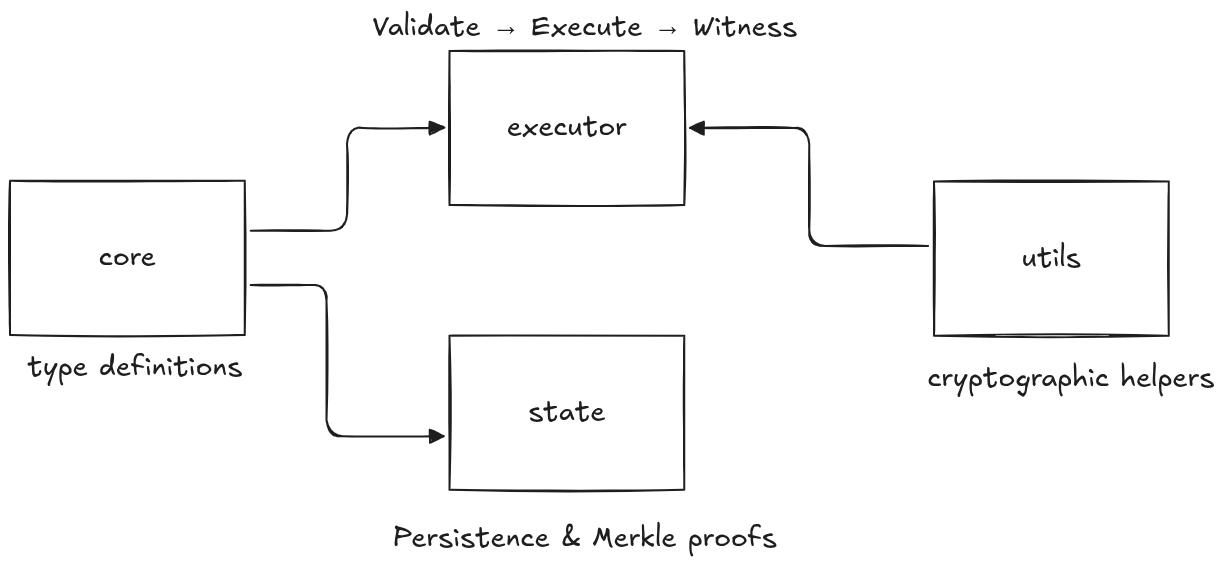
\includegraphics[width=0.75\linewidth]{figures/executor-component-dependency.png}
    \caption{Executor component dependency graph}
    \label{fig:dependency}
\end{figure}

Each module encapsulates a distinct responsibility boundary: core defines the domain vocabulary, executor implements state transition logic, state manages persistent storage with cryptographic commitments, and utils provides cross-cutting cryptographic primitives. This modularization enables independent optimization, testing, and potential substitution of components without cascading changes throughout the system.

\subsubsection{Architectural Components}
The executor architecture comprises four primary modules, each implementing specific design patterns to ensure extensibility and testability.

\subsubsubsection{Core Module (\texttt{src/core/})}

The core module serves as the foundational layer, defining shared types and behavioral contracts used throughout the system. It establishes the domain vocabulary and cryptographic primitives.

\paragraph{File Structure}
The module is organized into the following components:
\begin{itemize}[leftmargin=*, noitemsep]
    \item \texttt{types.rs}: Defines core data structures including \texttt{Account}, \texttt{Transaction}, \texttt{Receipt}, \texttt{Block}, and \texttt{Batch}.
    \item \texttt{command.rs}: Contains the \texttt{TransactionExecutor} trait.
    \item \texttt{rlp.rs}: Handles Ethereum-compatible RLP (Recursive Length Prefix) encoding.
    \item \texttt{batch.rs}: Utilities for processing transaction batches.
\end{itemize}

\paragraph{Key Abstractions}
The architecture relies on several primary types and a specific command pattern to handle state transitions.

\begin{description}[style=nextline, leftmargin=*]
    \item[Key Types] 
    Key data structures include:
    \begin{itemize}
        \item \texttt{Transaction}: Enum variants for \texttt{Transfer}, \texttt{ContractCall}, and \texttt{ContractCreate}. It utilizes \texttt{alloy-primitives} (\texttt{Address}, \texttt{U256}, \texttt{B256}) for Ethereum-native compatibility.
        \item \texttt{Account}: Manages balance, nonce, \texttt{code\_hash}, and \texttt{storage\_root}.
        \item \texttt{Receipt}: Stores execution results and emitted logs.
    \end{itemize}

    \item[The Command Pattern] 
    The \texttt{TransactionCommand} trait (Listing~\ref{lst:command}) encapsulates transaction-specific execution logic, enabling polymorphic handling of transaction variants.
\end{description}

\begin{lstlisting}[style=rustStyle, caption={The Transaction Command Trait}, label={lst:command}]
pub trait TransactionCommand {
    fn execute(&self, state: &mut StateManager, ...) -> Result<...>;
    fn sender(&self) -> &Address;
    // ... other methods
}
\end{lstlisting}

\paragraph{Implementations}
Concrete implementations of the command pattern include:
\begin{itemize}
    \item \textbf{TransferTx}: Handles native balance transfers between accounts.
    \item \textbf{ContractCallTx}: Executes EVM contract calls via the \texttt{EvmExecutor}.
    \item \textbf{ContractCreateTx}: Manages contract deployment logic via the \texttt{EvmExecutor}.
\end{itemize}

\subsubsubsection{Executor Module (\texttt{src/executor/})}

\begin{figure}[H]
    \centering
    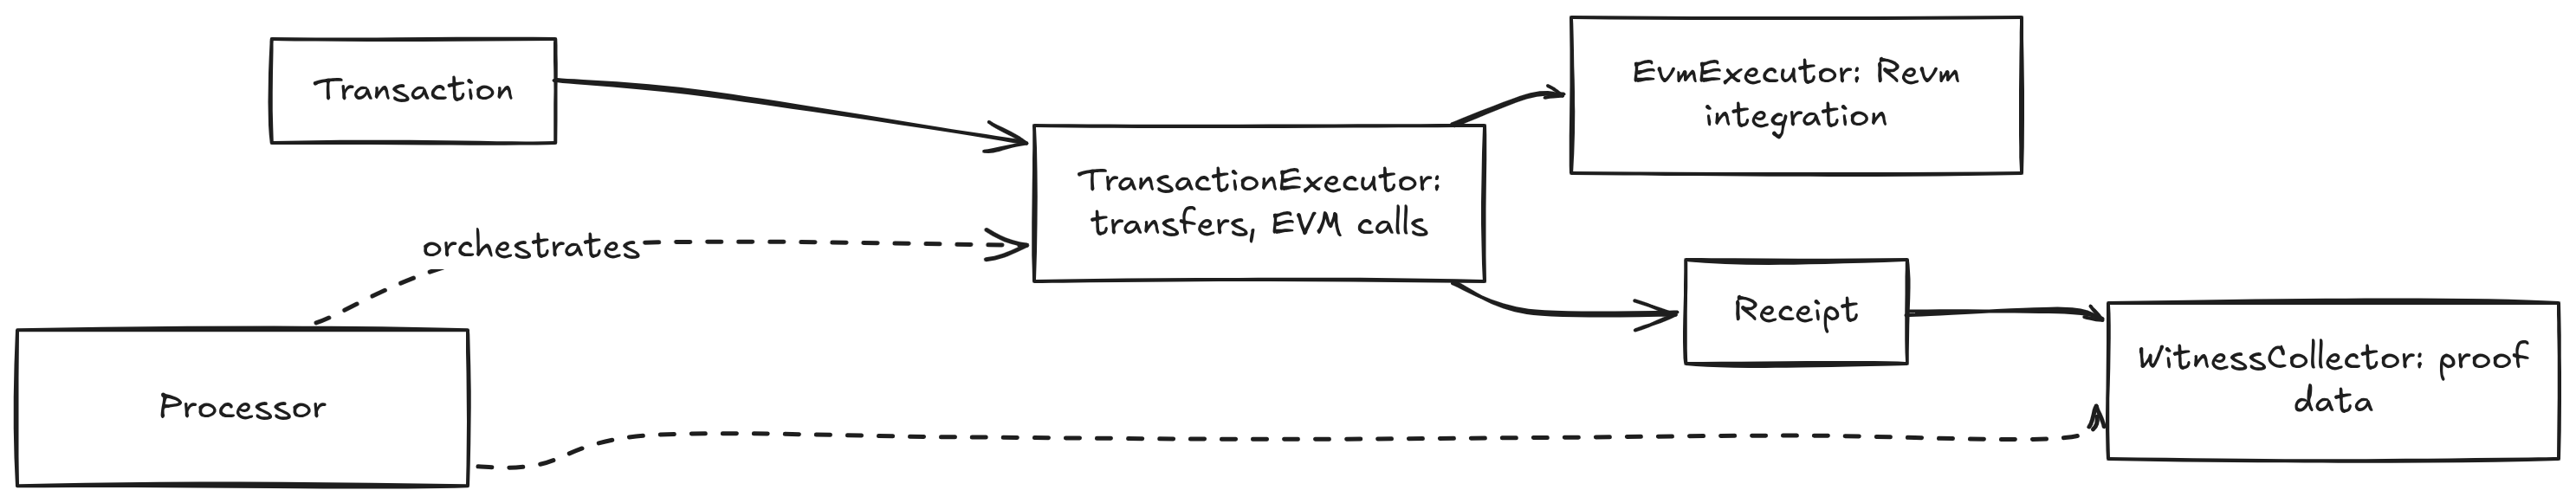
\includegraphics[width=0.75\linewidth]{figures/executor-executor.png}
    \caption{Executor executor module}
    \label{fig:tx_flow}
\end{figure}

The executor module constitutes the primary transaction processing engine. It adheres strictly to the Single Responsibility Principle, separating the concerns of transaction routing and EVM integration.

\paragraph{File Structure}
The module is organized into the following key components:
\begin{itemize}[leftmargin=*, noitemsep]
    \item \texttt{tx\_executor.rs}: Contains the \texttt{TransactionExecutor}, dispatching transactions to transfer logic or the EVM.
    \item \texttt{evm.rs}: Contains the \texttt{EvmExecutor}, which wraps the \textbf{revm} crate for smart contract execution.
    \item \texttt{processor.rs}: The main coordinator that owns the state manager and orchestrates block execution.
\end{itemize}

\paragraph{Key Components and Patterns}
The architecture utilizes several classical design patterns to manage execution complexity and abstract external dependencies.

\begin{description}[style=nextline, leftmargin=*]
    \item[Processor (Facade Pattern)] 
    Acts as the main coordinator for the entire execution subsystem. Clients interact with the \texttt{Processor}, which hides internal complexity, handles batch atomicity (all-or-nothing execution), and orchestrates the transaction lifecycle via methods like \texttt{execute\_transaction()} and \texttt{execute\_block()}.

    \item[TransactionExecutor (Strategy Pattern)] 
    Serves as the transaction dispatcher. It selects the appropriate execution strategy—either native balance transfers or EVM execution—based on the underlying transaction type.

    \item[EvmExecutor (Adapter Pattern)] 
    Acts as the dedicated execution engine. It bridges the internal \texttt{StateRepository} and \texttt{Transaction} types to the interfaces required by the \texttt{revm} crate (\texttt{Database}, \texttt{TxEnv}), safely configuring and running the Ethereum Virtual Machine.
\end{description}

\begin{lstlisting}[style=rustStyle, caption={The Transaction Executor Trait}, label={lst:executor}]
pub trait TransactionExecutor {
    fn execute(&self, state: &mut impl StateRepository) -> Result<Receipt>;
}
\end{lstlisting}

\subsubsubsection{State Module (\texttt{src/state/})}

\begin{figure}[H]
    \centering
    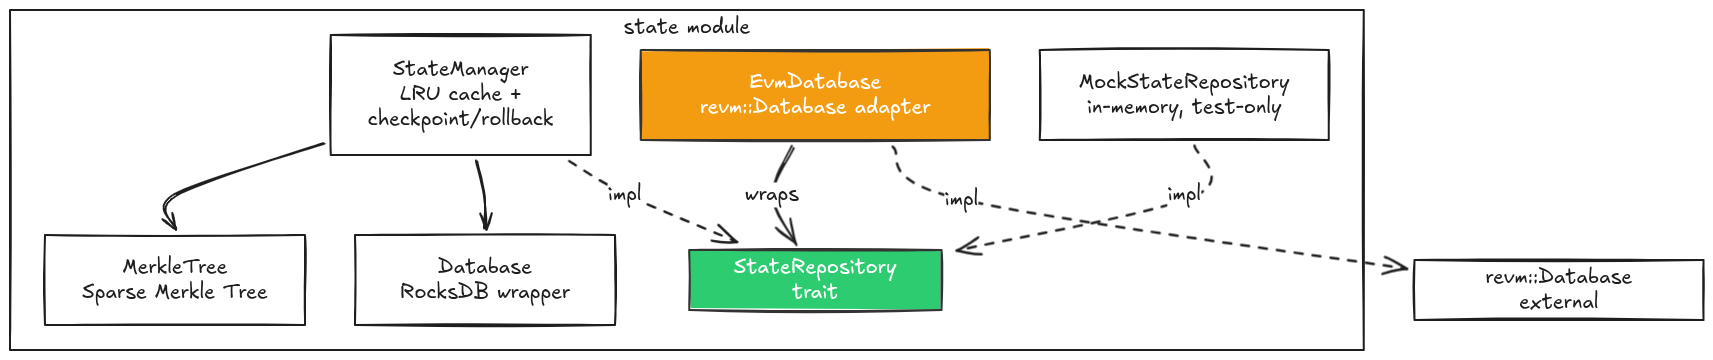
\includegraphics[width=0.75\linewidth]{figures/executor-state.png}
    \caption{Executor state module}
    \label{fig:tx_flow}
\end{figure}

The state module manages data persistence, cryptographic integrity, and efficient state access. It ensures crash consistency and leverages dependency inversion, guaranteeing that high-level execution modules depend on behavioral abstractions rather than concrete storage implementations.

\paragraph{File Structure}
The module is organized into the following components:
\begin{itemize}[leftmargin=*, noitemsep]
    \item \texttt{repository.rs}: Defines the core \texttt{StateRepository} trait.
    \item \texttt{manager.rs}: Contains \texttt{StateManager}, the primary implementation featuring LRU caching, checkpointing, and atomic commits.
    \item \texttt{storage/db.rs}: Provides the \texttt{Database} wrapper around RocksDB for persistent storage.
    \item \texttt{merkle/tree.rs}: Implements a Sparse Merkle Tree (Blake2b) for state root computation.
    \item \texttt{storage/evm\_db.rs}: Contains \texttt{EvmDatabase}, bridging the state manager to the EVM.
    \item \texttt{mock.rs}: Provides \texttt{MockStateRepository}, an in-memory HashMap implementation for testing.
\end{itemize}

\paragraph{Key Components and Patterns}
\begin{description}[style=nextline, leftmargin=*]
    \item[StateRepository (Repository Pattern)] 
    The central abstraction layer. It defines state access operations, allowing the execution logic to remain entirely agnostic to the underlying storage mechanism.

    \item[StateManager] 
    The main state controller implementing the repository trait. It combines Caching (LRU), Atomic Commit, and Snapshot/Restore patterns. It batches database writes to ensure the system never enters a partially updated state.

    \item[EvmDatabase (Adapter Pattern)] 
    Serves as a structural bridge between the internal \texttt{StateRepository} interface and the \texttt{revm::Database} trait.

    \item[MerkleTree] 
    Acts as the system's cryptographic accumulator. It maintains the state tree and generates the State Root, which serves as a verifiable cryptographic commitment to the entire Layer-2 state.
\end{description}

\begin{lstlisting}[style=rustStyle, caption={The State Repository Trait}, label={lst:repository}]
pub trait StateRepository {
    fn get_account(&mut self, addr: &Address) -> Result<Account>;
    fn update_account(&mut self, addr: &Address, account: Account) -> Result<()>;
    fn get_storage(&mut self, addr: &Address, key: &Hash) -> Result<Vec<u8>>;
    fn commit(&mut self) -> Result<Hash>;
    // ... additional storage methods
}
\end{lstlisting}

\subsubsubsection{Utils Module (\texttt{src/utils/})}

The utils module serves as a shared library of cross-cutting concerns, primarily focusing on essential cryptographic primitives and helper functions utilized throughout the entire execution engine. 

\paragraph{File Structure}
\begin{itemize}[leftmargin=*, noitemsep]
    \item \texttt{crypto.rs}: Contains core cryptographic utilities, including hashing and address derivation logic.
\end{itemize}

\paragraph{Key Components}
\begin{description}[style=nextline, leftmargin=*]
    \item[Hashing Operations] 
    Provides standard Ethereum-compatible hashing via \texttt{keccak256}, which is foundational for data integrity checks, state root generation, and transaction hashing.

    \item[Address Derivation] 
    Contains \texttt{public\_key\_to\_address} logic, mapping cryptographic public keys to standard 20-byte Ethereum addresses.
\end{description}

\subsubsection{Operational Flow}

\begin{figure}[H]
    \centering
    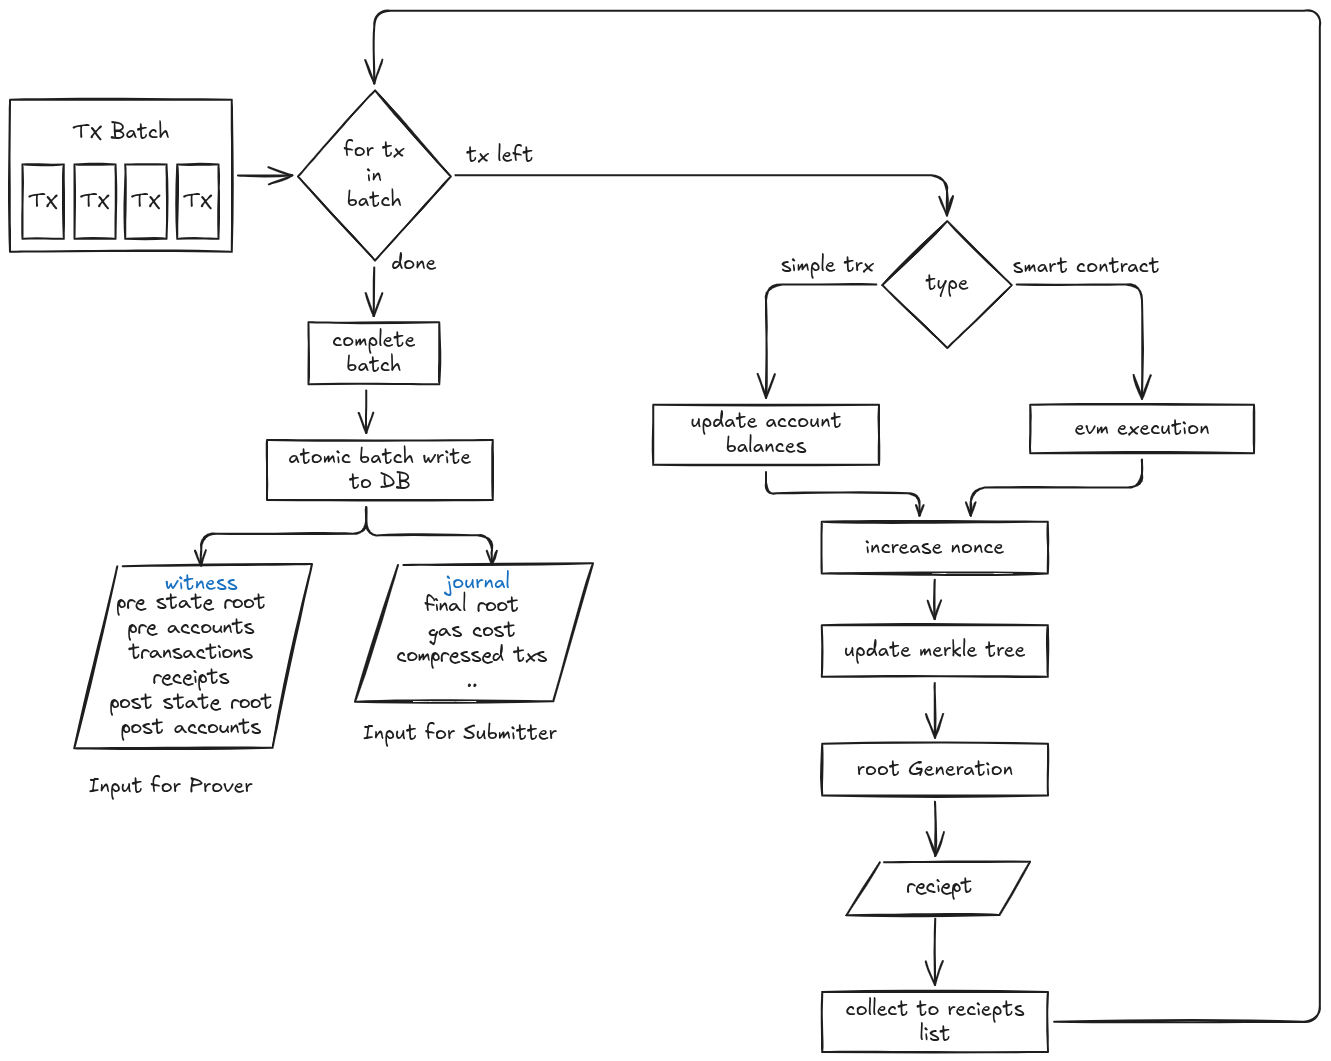
\includegraphics[width=0.75\linewidth]{figures/executor-tx-flow.png}
    \caption{Executor transaction flow}
    \label{fig:tx_flow}
\end{figure}

\begin{figure}[H]
    \centering
    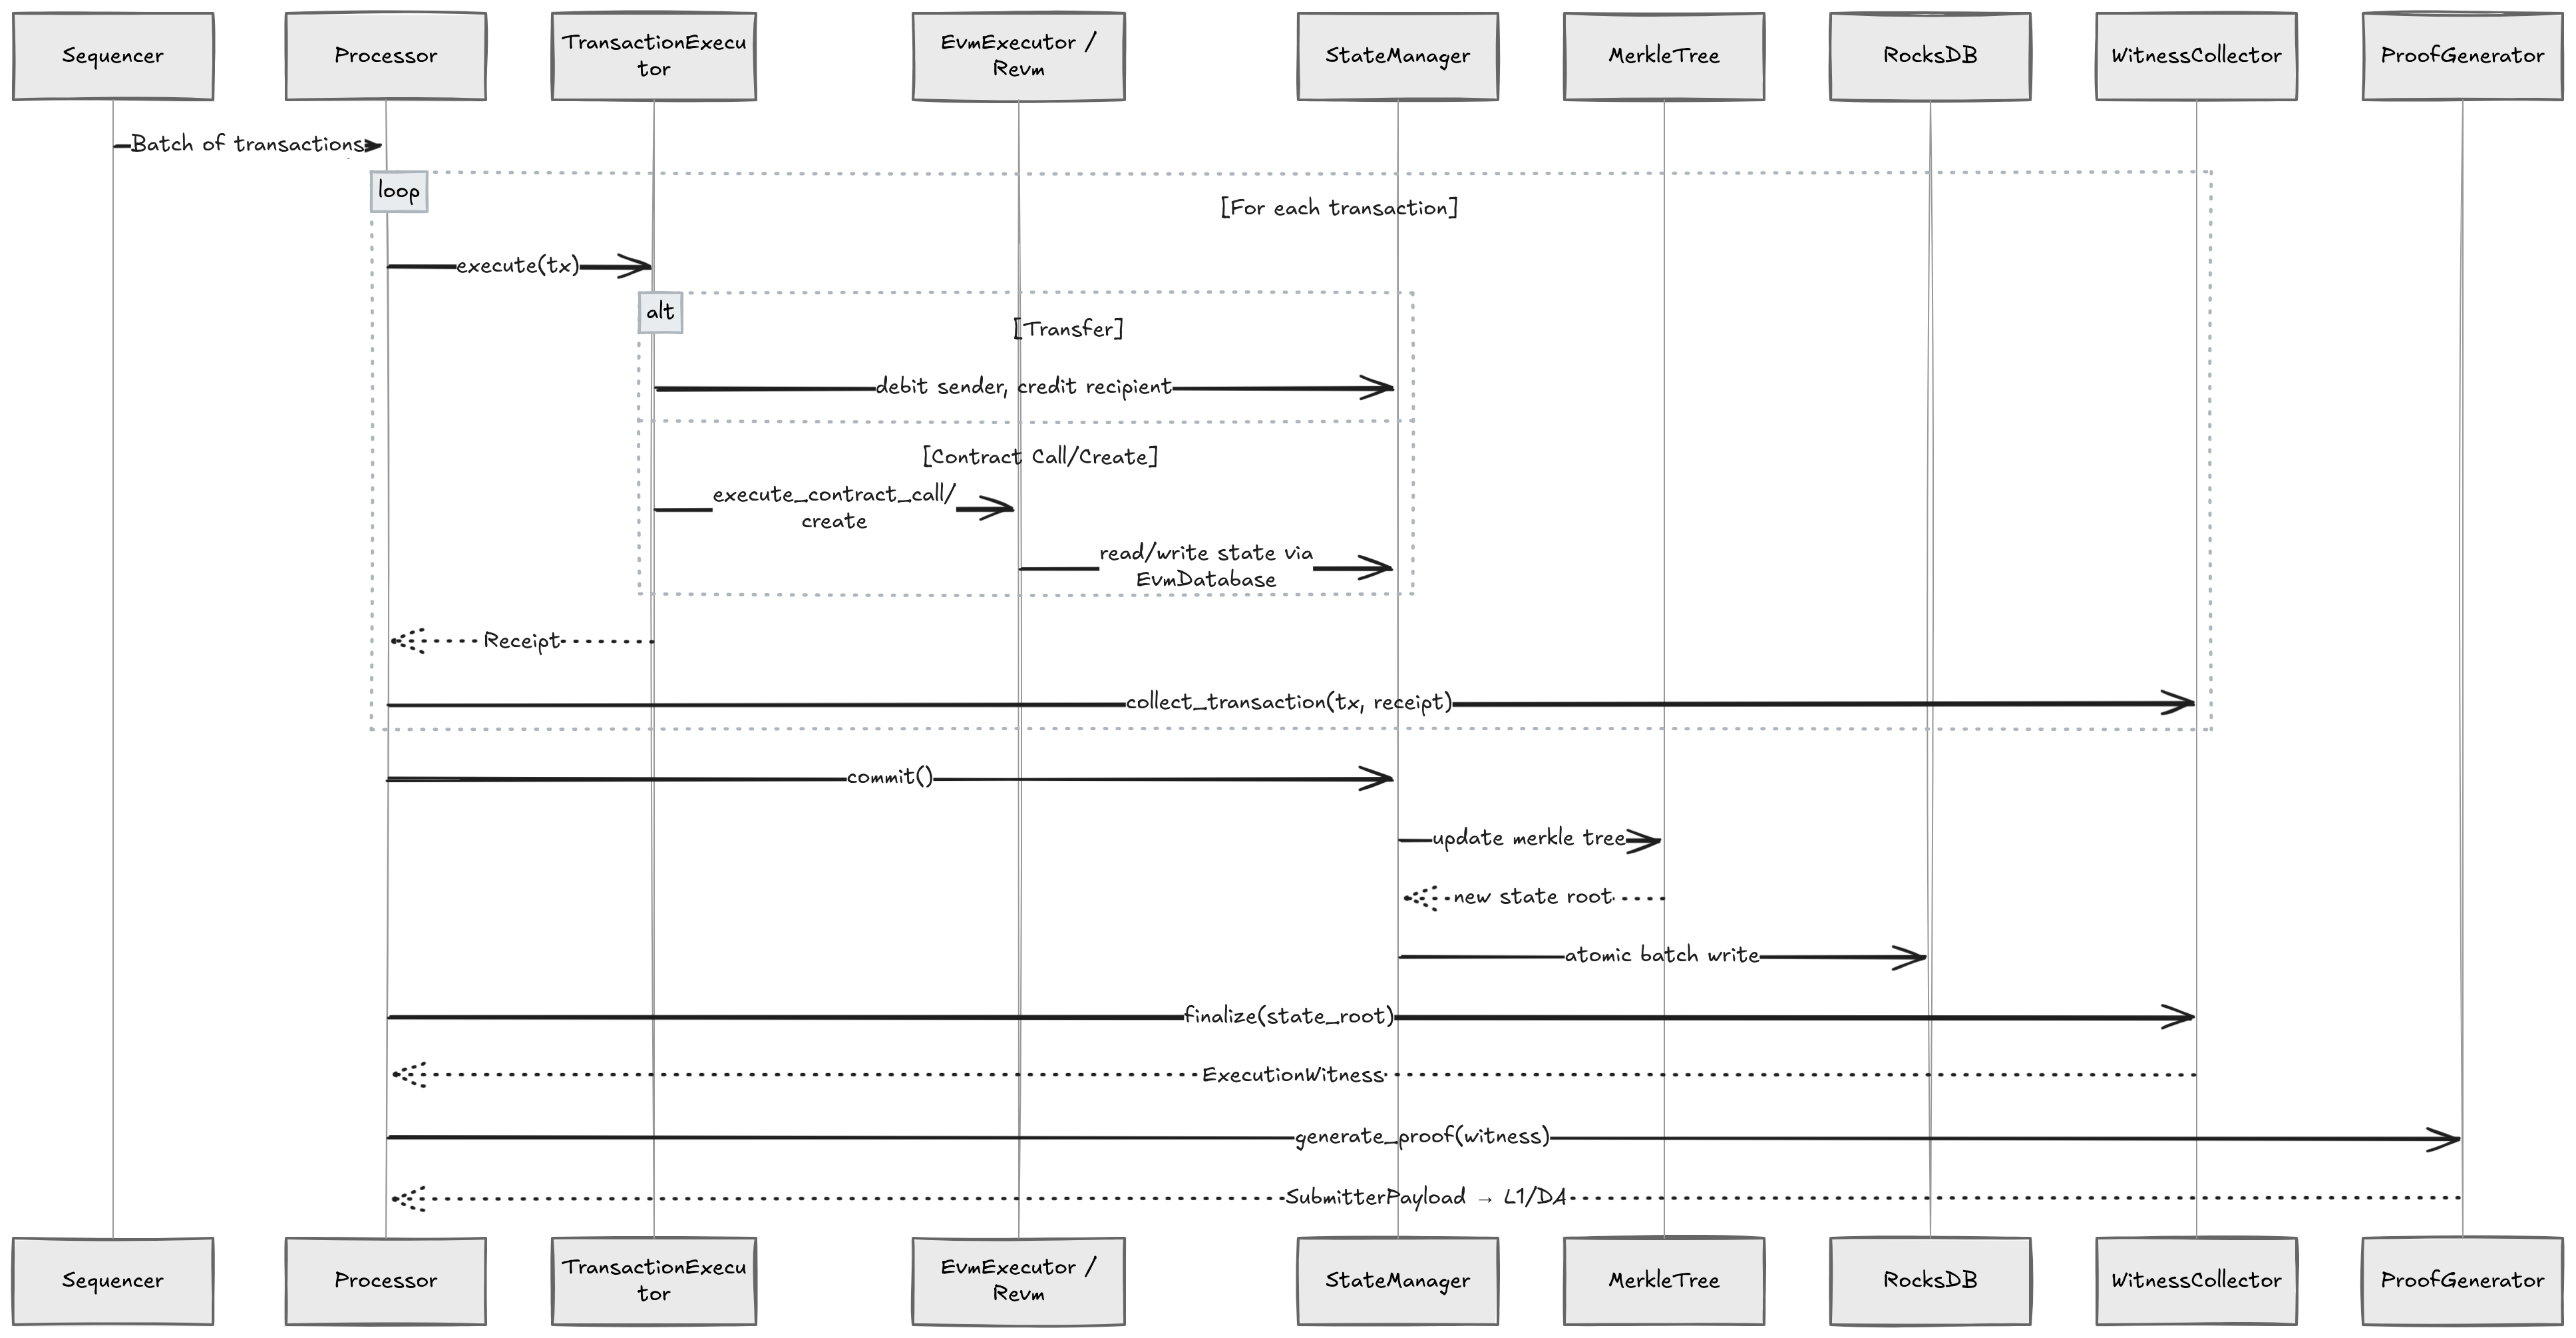
\includegraphics[width=0.75\linewidth]{figures/executor-flow.png}
    \caption{Executor sequence diagram}
    \label{fig:tx_flow}
\end{figure}

\paragraph{Phase 1: Execution (Executor Module)}
Transaction dispatch occurs based on type:
\begin{itemize}[leftmargin=*]
    \item \textbf{Transfer}: Direct state mutation via \texttt{StateRepository} (debit sender, credit recipient).
    \item \textbf{Contract Operations}: Delegation to \texttt{EvmExecutor}, which instantiates \texttt{revm::Evm} with an \texttt{EvmDatabase} adapter bridging to \texttt{StateRepository}.
\end{itemize}

\paragraph{Phase 2: State Commitment (State Module)}
Post-execution, \texttt{StateManager::commit()} performs:
\begin{enumerate}[leftmargin=*]
    \item Collection of dirty accounts from pending write set
    \item Serialization via \texttt{bincode}
    \item Merkle tree updates with new state root computation
    \item Atomic batch write to RocksDB (all-or-nothing persistence)
\end{enumerate}

\subsubsection{Design Rationale and Trade-offs}
\label{sec:rationale}

\paragraph{Modular Separation vs. Performance}
The strict module separation introduces interface overhead but yields critical benefits:
\begin{itemize}[leftmargin=*]
    \item \textbf{Testability}: Mock implementations enable unit testing without database instantiation ($<$1ms vs. disk I/O).
    \item \textbf{Swappability}: Storage engines (RocksDB $\rightarrow$ LMDB) are interchangeable without cascading changes.
    \item \textbf{Parallel Development}: Team members can own modules with minimal merge conflicts.
\end{itemize}

\paragraph{Alloy Primitives Adoption}
Standardizing on \texttt{alloy-primitives} (\texttt{Address}, \texttt{U256}, \texttt{B256}) rather than custom types:
\begin{itemize}[leftmargin=*]
    \item[\cmark] Zero-cost interop with \texttt{revm} (shared type system)
    \item[\cmark] Battle-tested 256-bit arithmetic (security critical)
    \item[\cmark] Native RLP encoding via \texttt{alloy-rlp}
    \item[\xmark] Dependency on external crate evolution
\end{itemize}

\paragraph{Revm Integration vs. Custom EVM}
Using \texttt{revm} rather than a custom EVM implementation:
\begin{itemize}[leftmargin=*]
    \item[\cmark] Production-tested (used by Reth, Foundry)
    \item[\cmark] Complete opcode and precompile support
    \item[\cmark] Trait-based \texttt{Database} interface enables state layer decoupling
    \item[\xmark] Binary size overhead
\end{itemize}

\paragraph{Sparse Merkle Tree Selection}
Blake2b-based SMT chosen over alternatives:
\begin{itemize}[leftmargin=*]
    \item[\cmark] Efficient for sparse key spaces (typical blockchain state)
    \item[\cmark] Faster than SHA-256 in most environments
    \item[\xmark] Less standard than SHA-256 for external verification
\end{itemize}

\paragraph{LRU Cache Sizing}
10K account / 50K storage slot cache limits represent a balance between:
\begin{itemize}[leftmargin=*]
    \item Hit rate optimization (typical block access patterns show locality)
    \item Memory constraints (bounded usage prevents OOM in long-running nodes)
    \item Checkpoint overhead (larger caches increase rollback memory)
\end{itemize}

\paragraph{Nonce Increment Timing}
Nonces increment \textit{after} execution:
\begin{itemize}[leftmargin=*]
    \item Matches Ethereum semantics where reverted transactions still consume nonces
    \item Requires careful handling of out-of-gas scenarios in EVM execution
\end{itemize}



\subsubsection{Integration with Other Components}
\label{sec:integration}

The executor crate interfaces with key external system categories, acting as the central state-transition engine within the broader Layer-2 architecture:

\paragraph{Sequencer Integration}
The sequencer submits transaction batches via the \texttt{Batch} struct:
\begin{itemize}[leftmargin=*]
    \item \textbf{Interface}: Binary serialization (\texttt{bincode}) over network transport.
    \item \textbf{Contract}: The sequencer guarantees transaction ordering and data availability; the executor guarantees deterministic execution and state transitions.
    \item \textbf{Backpressure}: Executor TPS vs. Sequencer ingestion rate is managed dynamically via block batch sizing.
\end{itemize}

\paragraph{Zero-Knowledge Prover Integration}
The executor acts as the host/witness generator for an external prover system (e.g., a decentralized prover network or dedicated zkVM hardware):
\begin{itemize}[leftmargin=*]
    \item \textbf{Data Handoff}: The executor constructs an \texttt{ExecutionWitness} containing pre/post state roots, transaction receipts, and all necessary Merkle inclusion proofs.
    \item \textbf{Adapter Pattern}: Specific prover SDKs (such as RISC Zero or SP1) are isolated behind generic adapter traits, preventing vendor lock-in and allowing seamless prover substitution.
    \item \textbf{Stateless Proving}: Because the witness contains all required cryptographic data, the external prover can deterministically verify the state transition without needing access to the executor's RocksDB database.
\end{itemize}

\paragraph{Data Availability Layer \& Layer-1}
Post-execution and proving, the system outputs data for on-chain storage and verification:
\begin{itemize}[leftmargin=*]
    \item \textbf{Journal}: Public inputs intended for the Layer-1 verifier contract (post-state root, block number, gas used) to update the rollup's canonical state.
    \item \textbf{Batch Data}: Compressed transaction data submitted to the Data Availability (DA) layer to ensure state reconstruction is always possible.
\end{itemize}

\begin{table}[H]
\centering
\caption{External Dependencies and Integration Points}
\label{tab:dependencies}
\begin{tabular}{@{}llll@{}}
\toprule
\textbf{Category} & \textbf{Crate} & \textbf{Version} & \textbf{Purpose} \\
\midrule
Ethereum Types & \texttt{alloy-primitives} & 0.6+ & Address, U256, B256 \\
RLP Encoding & \texttt{alloy-rlp} & 0.6+ & Transaction hashing \\
EVM Execution & \texttt{revm} & 8.0+ & Smart contract runtime \\
Cryptography & \texttt{tiny-keccak} & 2.0+ & Hashing \\
Storage & \texttt{rocksdb} & 0.21+ & Persistent KV store \\
Merkle Trees & \texttt{sparse-merkle-tree} & 0.6+ & State commitments \\
Serialization & \texttt{serde}, \texttt{bincode} & 1.0+, 1.3+ & Wire format \\
\bottomrule
\end{tabular}
\end{table}

The dependency stack prioritizes \textbf{pure Rust} implementations where possible to eliminate C FFI complications during cross-compilation, a critical requirement for generating compatible execution witnesses for RISC-V-based zkVM environments.

\subsection{Submitter}
\subsubsection{Overview}

The \textbf{Submitter} service is the system’s dedicated \textbf{Layer 2 to Layer 1 relay}, responsible for taking finalized L2 batch outputs (state transition artifacts and proof material) and committing them to Ethereum for settlement. In practical terms, it is the component that turns an off-chain state transition into an on-chain, verifiable update by constructing an L1 transaction, submitting it through an Ethereum client, and tracking confirmation until the batch is safely finalized. Implemented in \textbf{Rust}, the Submitter benefits from strict type safety and memory safety guarantees, and it uses an asynchronous execution model (\texttt{tokio}) to support continuous operation under sustained load while concurrently handling I/O-heavy tasks such as RPC calls, file access, and receipt monitoring.

A core engineering goal of this module is \textbf{operational reliability}: batches must not be lost, state roots must not be submitted inconsistently, and failures (RPC instability, transient errors, or reorgs) must be handled in a controlled manner. To achieve this, the Submitter is structured using the \textbf{Hexagonal Architecture} (Ports and Adapters) pattern. This design separates the \emph{application core}—the submission lifecycle, validation checks, and strategy selection—from infrastructure dependencies such as Ethereum RPC providers, transaction signing/broadcasting logic, and off-chain storage. As a result, the core logic can be reasoned about and tested independently, while concrete adapters can be swapped or extended without rewriting orchestration logic. This architectural separation is particularly important for a research PoC, where the submission pipeline must support multiple DA modes and evolve without destabilizing the batch-finalization workflow.

\subsubsection{Architectural Components}

\begin{figure}[htbp]
 \begin{adjustwidth}{0cm}{}
  \centering
  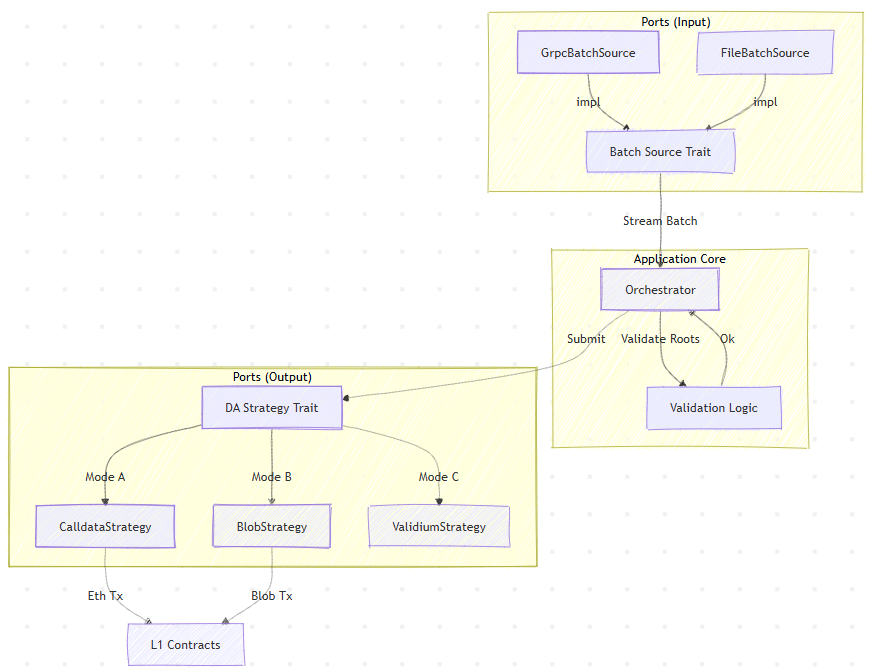
\includegraphics[width=0.95\linewidth]{figures/submitter-arch.png}
  \caption{Submitter architecture.}
  \label{fig:submitter-arch}
 \end{adjustwidth}
\end{figure}

As shown in Figure~\ref{fig:submitter-arch}, the Submitter is organized around a central \texttt{Orchestrator} (application core) surrounded by adapter modules that implement external interfaces (Ethereum client interaction, DA backends, compression, and storage). This structure makes the batch submission lifecycle explicit, while keeping environment-specific concerns isolated behind well-defined ports.

\subsubsubsection{Orchestrator (Core Logic)}

The \texttt{Orchestrator} is the primary control unit of the Submitter and manages the end-to-end lifecycle of a batch commitment attempt. It coordinates data movement and validation across all Submitter subcomponents, ensuring that only consistent and well-formed batch transitions are submitted to Layer 1. Concretely, the Orchestrator (i) \textbf{retrieves} the next available batch payload from the Executor via gRPC, (ii) performs \textbf{pre-submission consistency checks} to ensure the state roots and associated public inputs align before any on-chain action is taken, (iii) \textbf{selects} the active Data Availability mode based on runtime configuration, (iv) invokes the selected strategy to \textbf{construct and broadcast} the appropriate L1 transaction format, and (v) transitions into a \textbf{monitoring} state where transaction receipts are tracked until the required confirmation depth is reached.

The core loop, implemented in \texttt{daemon.rs}, continuously polls for new batches from the Executor/Prover interface (via gRPC) and processes them. The use of Rust's async/await pattern ensures that the service remains responsive even when waiting for long-running network operations like L1 block confirmations. Additionally, the orchestrator instruments every step of the process, capturing detailed performance metrics (latency, gas usage, confirmation blocks) into `SubmitterMetrics` for later analysis.

\begin{lstlisting}[style=rustStyle, caption={Submitter Orchestration Loop}, label={lst:submitter-loop}]
loop {
    match batch_source.next_batch().await {
        Ok(fetched) => {
            info!("Found new batch: {}", fetched.batch_id);
            // 1. Validation: Verify internal consistency of roots
            // ... (validation logic)

            // 2. Select DA Strategy (Polymorphism)
            match da_strategy.submit(&batch, &proof_hex, verifier_id).await {
                Ok(result) => {
                    info!("Batch submitted! Tx Hash: {}", result.tx_hash);
                    // 3. Metrics & Monitoring
                    save_metrics(result);
                }
                Err(e) => {
                    error!("Failed to submit batch: {}", e);
                    // Retry logic would be triggered here
                }
            }
        }
        Err(e) => {
            error!("Error fetching batch: {}", e);
            tokio::time::sleep(Duration::from_secs(5)).await;
        }
    }
}
\end{lstlisting}

In addition to successful submission, the Orchestrator is responsible for handling operational exceptions. It monitors for failed broadcasts, missing receipts, and network reorganizations, and it triggers appropriate recovery behavior so that the system can reach \emph{eventual finality} without manual intervention. This makes the Submitter a continuously running daemon rather than a one-shot relay script.

\subsubsubsection{DA Strategies (Adapters)}

To support systematic evaluation of DA cost and security trade-offs, the Submitter implements a configurable \texttt{DaStrategy} trait that abstracts how batch data is made available and how the on-chain contract is satisfied. Each DA mode is implemented as a concrete adapter module, allowing the Submitter to switch between strategies without modifying the orchestration path.

\begin{lstlisting}[style=rustStyle, caption={The Data Availability Strategy Trait}, label={lst:da-strategy}]
#[async_trait]
pub trait DaStrategy: Send + Sync {
    /// Prepares and submits the batch to L1
    async fn submit_batch(
        &self,
        batch_data: &BatchData,
        proof: &Proof
    ) -> Result<TxHash, SubmitterError>;

    /// Returns the mode identifier (0=Calldata, 1=Blob, 2=Validium)
    fn mode(&self) -> u8;
}
\end{lstlisting}

The strategy instantiation in \texttt{daemon.rs} demonstrates how the configuration drives the runtime behavior:

\begin{lstlisting}[style=rustStyle, caption={Dynamic DA Strategy Selection}, label={lst:da-strategy-selection}]
// Initialize DA Strategy based on Config
let da_strategy: Arc<dyn DaStrategy> = match cfg.da.mode {
    DaMode::Calldata => {
        let compression = cfg.aggregator.as_ref().and_then(|a| a.compression);
        Arc::new(CalldataStrategy::new(bridge.clone(), compression))
    },
    DaMode::Blob => {
        let archiver = cfg.da.archiver_url.clone();
        let default_hash = cfg.batch.blob_versioned_hash.as_deref().unwrap_or_default();
        let vh: H256 = default_hash.parse().unwrap_or_default();
        Arc::new(BlobStrategy::new(bridge.clone(), vh, idx, use_opcode, archiver))
    },
    DaMode::OffChain => {
        Arc::new(OffChainStrategy::new(bridge.clone()))
    }
};
\end{lstlisting}

\paragraph{Mode A: Calldata (Maximum Security)}
Implemented in \texttt{infrastructure/da\_calldata.rs}, this strategy posts the full batch payload directly to Ethereum transaction calldata. Because calldata is permanently replicated as part of Ethereum history, it provides the strongest availability guarantees and simplest verification assumptions. The trade-off is cost: calldata incurs high per-byte gas overhead (16 gas per byte), which makes this mode expensive for large batches and serves as a baseline for cost comparison.

\paragraph{Mode B: Blobs / EIP-4844 (Cost Optimized)}
Implemented in \texttt{infrastructure/da\_blob.rs}, this strategy uses EIP-4844 \textbf{blob transactions} (Type 3) introduced with the Dencun upgrade. By placing data into the blob data space rather than permanent calldata, the strategy reduces on-chain data cost while still providing availability within the blob retention window (approximately 18 days). The implementation encapsulates blob-specific responsibilities such as blob construction, versioned hash generation, and sidecar propagation (often supported by an external Archiver for payload handling). This mode is designed to represent a practical cost/performance optimization while remaining compatible with Ethereum settlement.

\begin{lstlisting}[style=rustStyle, caption={Blob strategy submission logic}, label={lst:blob-submit}]
async fn submit(
    &self,
    batch: &Batch,
    proof_hex: &str,
    verifier_id: u8,
) -> Result<SubmissionResult, DomainError> {
    // 1. Read & Compress Payload
    let data = std::fs::read(&batch.data_file)?;
    let (payload_data, metrics) = CompressionStrategy::compress(&data);

    // 2. Archiver: POST data to external service (Sidecar emulation)
    if let Some(url) = &self.archiver_url {
        // ... (HTTP POST to archiver) ...
    }

    // 3. Construct EIP-4844 Transaction
    let tx_req = Eip1559TransactionRequest::new()
        .to(self.bridge.address())
        .data(calldata); // Contains only commitment, not data

    // ... (Signing and Broadcast) ...
}
\end{lstlisting}

\paragraph{Mode C: Off-Chain / Validium (Lowest Cost)}
Implemented in \texttt{infrastructure/da\_offchain.rs}, this strategy stores the batch data externally and posts only a compact \textbf{data commitment} (CID/hash) to the L1 contract. This achieves minimal on-chain data cost but introduces an explicit availability trust assumption on the external data layer. In the current PoC, a local filesystem path (\texttt{offchain\_store/}) is used as the off-chain storage backend to prototype the integration pattern for decentralized storage systems such as IPFS or Celestia.

\subsubsubsection{Compression Strategy}

To further reduce on-chain data footprint where applicable, the Submitter includes a dedicated \texttt{CompressionStrategy} module (\texttt{infrastructure/compression.rs}). This module implements a \textbf{bit-packing} approach for transaction payloads by converting structured transaction data into a compact binary representation. The strategy removes JSON encoding overhead and enforces consistent field encoding (for example, normalizing numeric encodings such as removing leading zeros) to improve density. During operation, the module computes benchmarking metrics such as \texttt{compression\_ratio} and \texttt{gas\_saved}, enabling experimental comparison between raw submission and compressed submission under identical workloads.

\begin{lstlisting}[style=rustStyle, caption={Bit-Packing Compression Logic}, label={lst:compression-logic}]
fn bit_pack_transactions(txs: &[Value]) -> Vec<u8> {
    let mut buffer = Vec::new();
    buffer.push(0x01); // Version Byte

    for tx in txs {
        // ... (Field extraction)

        // Bit Packing:
        // 1. From (20 bytes)
        buffer.extend_from_slice(&from);

        // 2. To (20 bytes)
        buffer.extend_from_slice(&to);

        // 3. Amount (VarInt - remove leading zeros)
        let mut start = 0;
        while start < 32 && value[start] == 0 {
            start += 1;
        }
        let len = 32 - start;
        buffer.push(len as u8);
        buffer.extend_from_slice(&value[start..]);

        // 4. Nonce (VarInt)
        // ... (Nonce packing similar to Amount)

        // 5. Signature (65 bytes)
        buffer.extend_from_slice(&[0u8; 65]);
    }
    buffer
}
\end{lstlisting}

\subsubsubsection{Submitter Data Model}

The Submitter maintains persistent batch-level state to support safe recovery and controlled retries. This includes tracking the batch identifier, status, selected DA mode, submission attempts, and the corresponding L1 transaction hash.

\begin{figure}[htbp]
 \begin{adjustwidth}{0cm}{}
  \centering
  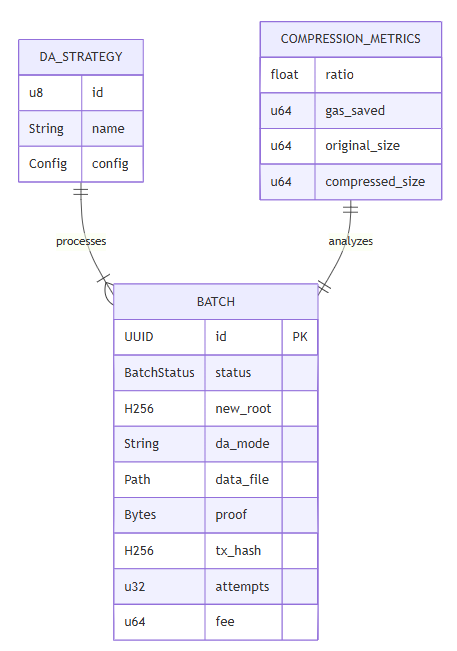
\includegraphics[width=0.95\linewidth]{figures/submitter-er.png}
  \caption{Submitter ER Diagram.}
  \label{fig:submitter-er}
 \end{adjustwidth}
\end{figure}

Figure~\ref{fig:submitter-er} summarizes the Submitter’s persistence model, centered around the \texttt{Batch} entity and its relationships to DA strategy selection and compression metrics. This persisted metadata is essential for robustness: it enables the service to restart without losing submission progress and provides a concrete audit trail of batch handling decisions, including retry behavior and final submission outcomes.

\subsubsection{Operational Sequence}

\begin{figure}[htbp]
 \begin{adjustwidth}{0cm}{}
  \centering
  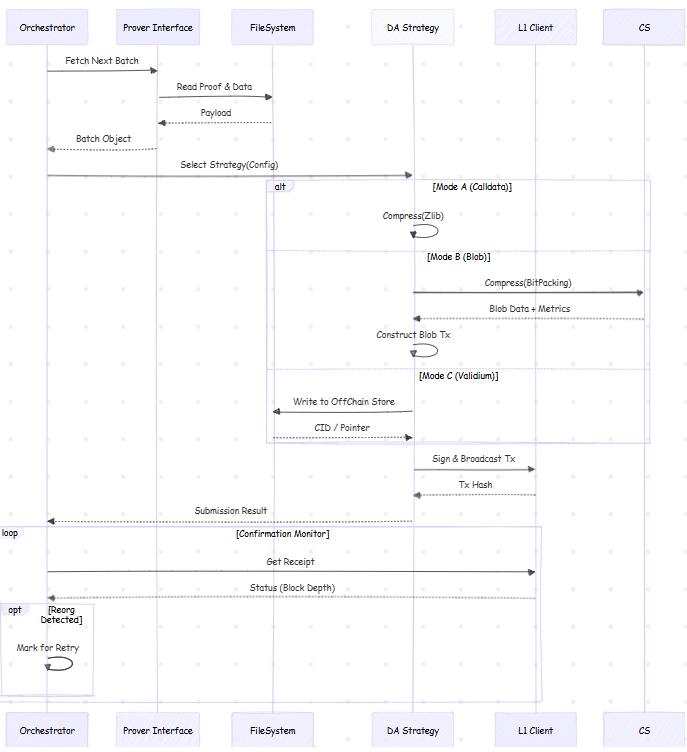
\includegraphics[width=0.95\linewidth]{figures/submitter-seq.png}
  \caption{Submitter Operational Sequence.}
  \label{fig:submitter-seq}
 \end{adjustwidth}
\end{figure}

The Submitter operates as a deterministic pipeline whose primary objective is to preserve data integrity while ensuring successful settlement. As depicted in Figure~\ref{fig:submitter-seq}, the sequence proceeds as follows. The Orchestrator first \textbf{fetches} the next batch payload from the Executor/Prover interface and performs pre-submission validation to ensure the provided roots and public inputs are internally consistent. It then \textbf{selects} the configured DA strategy (Calldata, Blob, or Validium). Where applicable (notably in data-heavy modes), the payload is \textbf{compressed} using the bit-packing strategy to minimize on-chain footprint and enable quantitative benchmarking of size reduction. Next, the selected adapter \textbf{constructs and submits} the appropriate L1 transaction format—Legacy or EIP-1559 for calldata-based modes, and Type 3 transactions for blob-based mode—using the Ethereum client adapter for signing and broadcast. Finally, the Submitter enters a \textbf{confirmation monitoring} phase, continuously polling for receipts, detecting reorganizations, and only marking the batch as confirmed once the configured confirmation depth is reached.

This operational design ensures that submission is not treated as a best-effort broadcast, but as a controlled finalization protocol that remains robust under realistic Ethereum network conditions.

\subsubsection{Design Rationale and Trade-offs}

\paragraph{Hexagonal Architecture}
The choice of Hexagonal Architecture (Ports and Adapters) allows for extreme configurability. The \texttt{Orchestrator} remains unaware of whether it is posting to a local testnet, Sepolia, or using blobs. This was crucial for iterative development, allowing the DA layer to evolve from simple calldata to complex EIP-4844 blobs without rewriting the core loop.

\paragraph{Bit-Packing vs. RLP}
While RLP is standard, the custom bit-packing strategy (Listing~\ref{lst:compression-logic}) was chosen to maximize data density for DA. By removing JSON overhead and using variable-length integer encoding, we achieved significant cost reductions (approx. 40\%) compared to raw JSON submission, which is critical for the economic feasibility of the rollup.

\paragraph{Polymorphic DA Strategies}
Implementing DA strategies as a trait (Listing~\ref{lst:da-strategy}) enables the system to adapt to different security/cost requirements at runtime. This "Strategy Pattern" mirrors the one used in the Smart Contracts, ensuring consistency across the off-chain and on-chain components.

\paragraph{Experimental Rigor}
To support the scientific goals of this project, the Submitter includes features specifically for benchmarking and analysis. This includes a "Mock Verification" mode (implemented in the \texttt{Orchestrator}) that bypasses on-chain calls to isolate measuring prover performance, and detailed \texttt{SubmitterMetrics} collection (latency, gas costs, block confirmations) which are serialized for post-hoc evaluation.


\subsection{Prover}
\subsubsection{Overview}

The \textbf{RollupX Prototype Prover} is a \textbf{zk-Rollup (Zero-Knowledge Rollup)} scaling solution for Ethereum. Its primary purpose is to enable \textbf{low-gas transfers of ETH and ERC-20 tokens} by moving transaction execution off-chain (Layer 2) while preserving the security guarantees of the Ethereum mainnet (Layer 1) through \textbf{cryptographic validity proofs}.

The core idea is simple: instead of processing every transaction on Ethereum directly, transactions are batched off-chain into \textbf{blocks}, a \textbf{zero-knowledge proof} is generated to attest to the correctness of all those transactions, and only the compact proof plus a small amount of public data is submitted on-chain. The Ethereum smart contract verifies the proof and updates the state without re-executing the transactions.

The system uses a \textbf{PLONK} proof system as an universal, succinct, non-interactive argument of knowledge (SNARK) backed by \textbf{Kate/KZG polynomial commitments} over the BN256 elliptic curve.

\subsubsection{System Components (Broad View)}

The system consists of three principal components that interact to form the full rollup pipeline:

\paragraph{Rollup Smart Contract (L1  Solidity)}

Located in \texttt{contracts/contracts/rollup.sol} and \texttt{contracts/contracts/PlonkCore.sol}, this is the on-chain anchor. It:
\begin{itemize}
    \item Manages user \textbf{balances} and \textbf{account state} on Ethereum.
    \item Accepts \textbf{priority operations} from L1 (e.g., \texttt{Deposit}, \texttt{FullExit}).
    \item \textbf{Commits} blocks by verifying their data integrity and storing block hashes.
    \item \textbf{Verifies PLONK proofs} (both single and recursive/aggregated) submitted by the server.
    \item \textbf{Executes} proven blocks to finalise withdrawals and state changes.
\end{itemize}

\paragraph{Server Application (L2  Rust)}

The server is the L2 node that orchestrates the rollup network. It exists in monolithic (\texttt{core/bin/server}) or microservice form:

\begin{table}[h]
\centering
\begin{tabular}{lll}
\toprule
\textbf{Microservice} & \textbf{Path} & \textbf{Responsibility} \\
\midrule
\textbf{Core} & \texttt{core/bin/Rollup\_core} & Mempool management,block generate \\
\textbf{API} & \texttt{core/bin/Rollup\_api} & REST API \& JSON RPC (HTTP) \\
\textbf{Ethereum Sender} & \texttt{core/bin/Rollup\_eth\_sender} & Submits prove/execute tx to L1 \\
\textbf{Witness Generator} & \texttt{core/bin/Rollup\_witness\_generator} & Builds circuit witness data;prover API \\
\bottomrule
\end{tabular}
\end{table}

\paragraph{Prover Application (Off-chain Worker Rust)}

Located in \texttt{core/bin/prover}, the prover is the computationally-intensive worker that generates zk-SNARK proofs. It polls the server for jobs, generates proofs, and returns results. Multiple provers can run concurrently for horizontal scalability.

\subsubsection{Transaction Lifecycle : Step-by-Step}

The following outlines how a transaction flows through the system from submission to finality:

\begin{verbatim}
 User submits Tx (L2)
        |
        |
        |
        v
┌──────────────────┐
│   Server (Core)   │         ← Accepts tx, validates, adds to mempool
│  Block Assembly   │         ← Groups txs into a block (with pubdata)
└──────────────────┘
        |
        |
        |
        v
┌──────────────────────────┐
│   Witness Generator       │ ← Builds circuit witness (account tree + ops)
│  (Prover Server API)     │  ← Stores witness in DB, serves it to provers
└──────────────────────────┘
        |
        |
        |
        v
┌──────────────────────────┐
│   Prover Worker           │ ← Polls for job, receives witness
│  (PlonkStepByStepProver) │  ← Generates PLONK single proof
│                          │  ← Generates aggregated recursive proof
└──────────────────────────┘
        |
        | 
        |
        v
┌──────────────────────────┐
│   Ethereum Sender         │ ← commitBlocks() → proveBlocks() → executeBlocks()
│  → L1 Smart Contract     │  ← On-chain verification via PlonkCore.sol
└──────────────────────────┘
\end{verbatim}

\textbf{Step 1 --- Transaction Submission:} Users submit L2 transactions (\texttt{Transfer}, \texttt{Withdraw}, \texttt{ChangePubKey}, \texttt{ForcedExit}) or trigger L1 priority operations (\texttt{Deposit}, \texttt{FullExit}).

\textbf{Step 2 --- Block Assembly:} The server's Core service batches transactions into blocks, applying state changes to the account tree.

\textbf{Step 3 --- Witness Generation:}  The Witness Generator loads the circuit account tree, applies each operation to build the \textbf{circuit witness} data, and stores it in the database.

\textbf{Step 4 --- Proof Generation:}  A Prover worker fetches the witness, generates a PLONK single proof per block, then aggregates proofs using a recursive circuit.

\textbf{Step 5 --- On-chain Finalization:}  The Ethereum Sender commits the block data on-chain, submits the aggregated proof, and upon successful verification the block is executed (withdrawals processed, state finalized).

\begin{figure}[htbp]
    \centering
    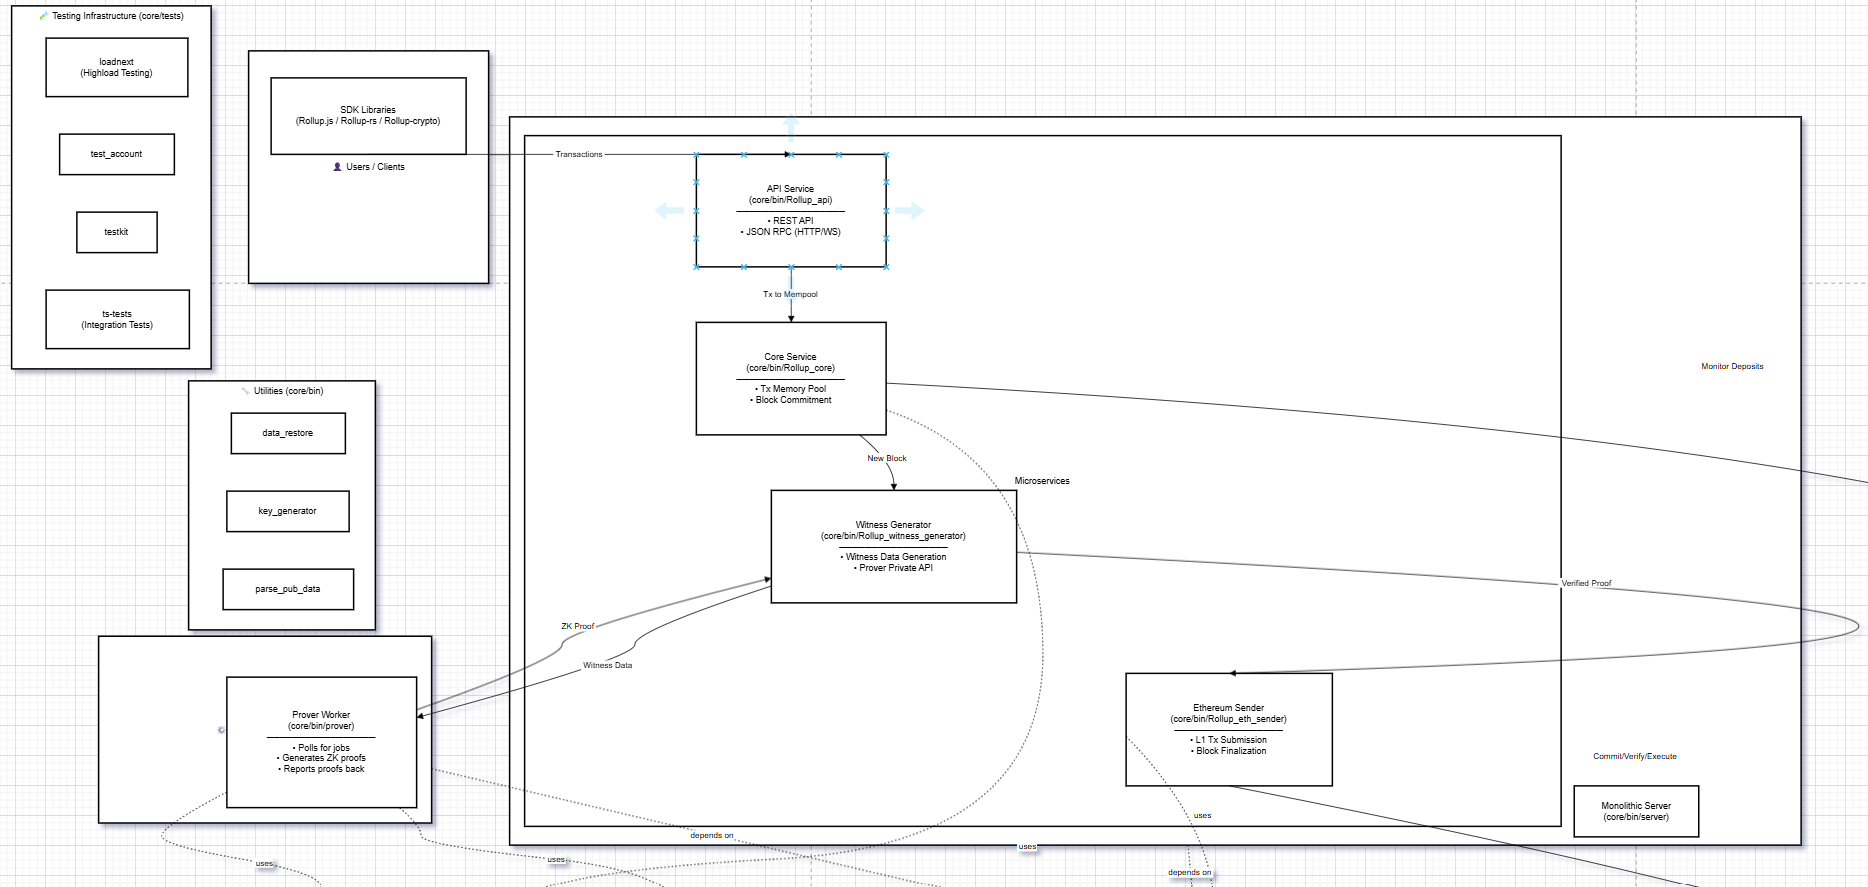
\includegraphics[width=0.9\textwidth]{figures/Diagram -1.png}
\end{figure}
\begin{figure}[htbp]
    \centering
    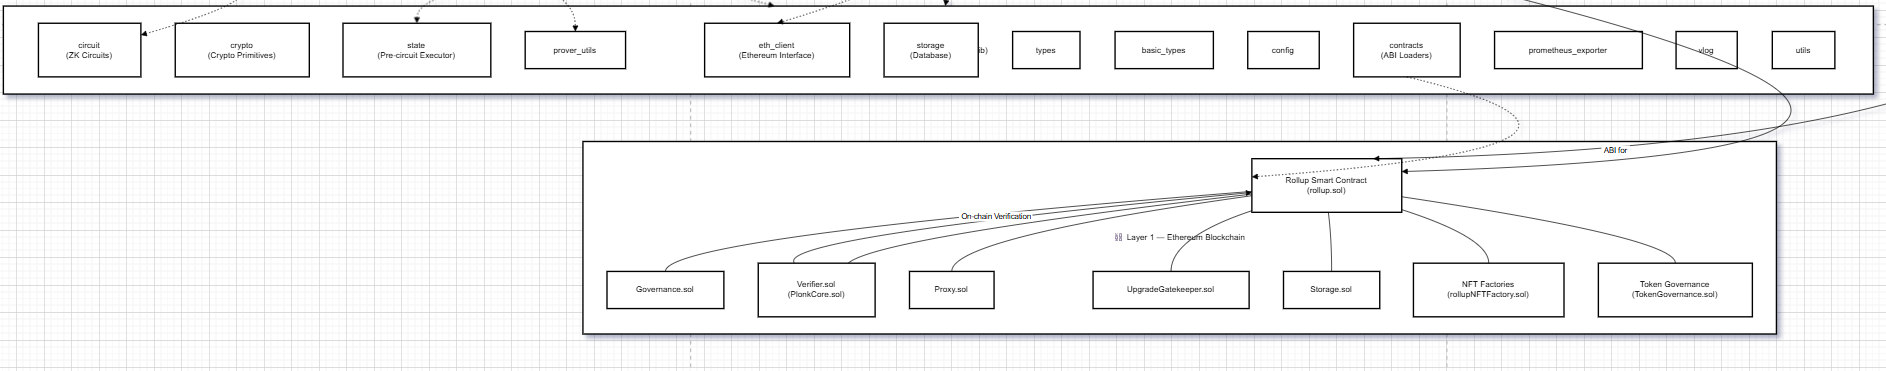
\includegraphics[width=0.9\textwidth]{figures/Daiagram -2.png}
    \caption{RollupX Prover Architecture showing the interaction between 
             Witness Generator, Prover Worker, and Ethereum contracts}
    \label{fig:prover-architecture}
\end{figure}

\subsubsection{The Prover --- Deep Dive}

\paragraph{Architecture \& Traits}

The prover system is built around two key Rust traits defined in \texttt{core/bin/prover/src/lib.rs}:

\begin{lstlisting}[caption={Core prover traits from \texttt{core/lib/prover\_utils/src/lib.rs}}]
/// Trait that provides type needed by prover to initialize.
pub trait ProverConfig {
    fn from_env() -> Self;
}

/// Trait that tries to separate prover from networking (API)
pub trait ProverImpl {
    type Config: ProverConfig;
    fn create_from_config(config: Self::Config) -> Self;
    fn get_request_aux_data(&self) -> ProverInputRequestAuxData { ... }
    /// Resource heavy operation
    fn create_proof(&self, data: JobRequestData) -> anyhow::Result<JobResultData>;
}
\end{lstlisting}

This trait-based design decouples proof logic from networking, allowing two interchangeable implementations:

\begin{table}[h]
\centering
\begin{tabular}{lll}
\toprule
\textbf{Implementation} & \textbf{File} & \textbf{Purpose} \\
\midrule
\texttt{PlonkStepByStepProver} & \texttt{core/bin/prover/src/plonk\_step\_by\_step\_prover.rs} & PLONK proofs \\
\texttt{DummyProver} & \texttt{core/bin/prover/src/dummy\_prover.rs} & Testing prover --- returns precomputed proofs \\
\bottomrule
\end{tabular}
\end{table}

\paragraph{Prover Work Cycle}

The main event loop is in \texttt{prover\_work\_cycle} (\texttt{core/bin/prover/src/lib.rs}):

\begin{enumerate}
    \item \textbf{Register} with the server via the API client.
    \item \textbf{Poll} the server's Witness Generator API (\texttt{get\_job}) for an idle prover job.
    \item \textbf{Receive} either a \texttt{BlockProof} job (single block witness) or an \texttt{AggregatedBlockProof} job (multiple single proofs to aggregate).
    \item \textbf{Compute} the proof on a blocking thread (via \texttt{compute\_proof\_no\_blocking}).
    \item \textbf{Send heartbeats} concurrently to keep the job alive while computing.
    \item \textbf{Publish} the result back to the server (\texttt{publish} endpoint).
    \item Repeat until shutdown.
\end{enumerate}

\vspace{5mm}
\paragraph{Prover Components}

The prover's internal components span multiple crates:

\subparagraph{Circuit (\texttt{core/lib/circuit})}

Defines the \textbf{ZkSyncCircuit} --- the arithmetic circuit that enforces transaction correctness. Key elements:

\begin{itemize}
    \item \textbf{\texttt{ZkSyncCircuit}} (\texttt{core/lib/circuit/src/circuit.rs}): The main circuit implementing \texttt{Circuit<E>}. It synthesizes constraints for every operation in a block, with a single public input: the \texttt{pub\_data\_commitment}.
    \item \textbf{\texttt{Witness} trait} (\texttt{core/lib/circuit/src/witness/mod.rs}): Each operation type (Deposit, Transfer, Withdraw, etc.) implements this trait to generate witness data by applying the operation to a \texttt{CircuitAccountTree}.
    \item \textbf{Operation-specific witnesses} (\texttt{core/lib/circuit/src/witness/\{deposit, transfer, withdraw, ...\}.rs}): Implements state transition logic for each zkSync operation.
\end{itemize}

\subparagraph{Crypto Primitives (\texttt{core/lib/crypto})}

Cryptographic foundations:

\begin{itemize}
    \item \textbf{Proof types} (\texttt{core/lib/crypto/src/proof.rs}): Defines \texttt{SingleProof} (PLONK proof for one block) and \texttt{AggregatedProof} (recursive proof aggregating multiple single proofs), along with their encoded/serialized forms for on-chain submission.
    \item \textbf{BN256 elliptic curve} operations, Rescue hash functions, and EdDSA signature verification.
\end{itemize}

\subparagraph{Prover Utils (\texttt{core/lib/prover\_utils})}

The engine room for proof generation:

\begin{itemize}
    \item \textbf{\texttt{SetupForStepByStepProver}} (\texttt{core/lib/prover\_utils/src/lib.rs}): Prepares the PLONK proving setup:
\end{itemize}

\begin{lstlisting}[language=Rust,caption={Setup structure from \texttt{core/lib/prover\_utils/src/lib.rs}}]
pub struct SetupForStepByStepProver {
    setup_polynomials: SetupPolynomials<Engine, PlonkCsWidth4WithNextStepParams>,
    hints: Vec<(usize, TranspilationVariant)>,
    setup_power_of_two: u32,
    key_monomial_form: Option<Crs<Engine, CrsForMonomialForm>>,
}
\end{lstlisting}

\begin{itemize}
    \item \textbf{\texttt{PlonkVerificationKey}}: Reads and caches per-block-size verification keys.
    \item \textbf{\texttt{aggregated\_proofs}} module (\texttt{core/lib/prover\_utils/src/aggregated\_proofs.rs}): Handles recursive proof aggregation.
\end{itemize}

\paragraph{Key Generator (\texttt{core/bin/key\_generator})}

A one-time utility that generates:

\begin{itemize}
    \item PLONK verification keys for each supported block size.
    \item Recursive aggregation verification keys.
    \item Sample/precomputed proofs for testing.
    \item The on-chain \textbf{Verifier contract} (auto-generated Solidity with embedded VKs).
\end{itemize}

\paragraph{How Proof Generation Works}
\paragraph{Step A --- Setup Preparation}

The prover prepares the PLONK proving setup by transpiling the circuit, computing setup polynomials, and loading the Common Reference String.


\begin{lstlisting}[caption={Setup preparation from \texttt{core/lib/prover\_utils/src/lib.rs}}]
impl SetupForStepByStepProver {
    pub fn prepare_setup_for_step_by_step_prover<C: Circuit<Engine> + Clone>(
        circuit: C,
        download_setup_file: bool,
    ) -> Result<Self, anyhow::Error> {
        let hints = transpile(circuit.clone())?;           // Transpile circuit to PLONK gates
        let setup_polynomials = setup(circuit, &hints)?;   // Compute setup polynomials
        let size = setup_polynomials.n.next_power_of_two().trailing_zeros();
        let setup_power_of_two = std::cmp::max(size, SETUP_MIN_POW2);
        let key_monomial_form = Some(get_universal_setup_monomial_form(
            setup_power_of_two, download_setup_file,
        )?);                                                // Load CRS (trusted setup)
        Ok(SetupForStepByStepProver { setup_polynomials, hints, setup_power_of_two, key_monomial_form })
    }
}
\end{lstlisting}

\begin{enumerate}
    \item \textbf{Transpile} the circuit into a PLONK-compatible gate representation (width-4 with next-step parameters).
    \item \textbf{Compute setup polynomials} (selector/permutation polynomials from the constraint system).
    \item \textbf{Load the CRS} (Common Reference String / Universal Setup) in monomial form from disk or network (power of two ranges from $2^{20}$ to $2^{26}$).
\end{enumerate}

\paragraph{Step B --- Single Proof Generation}

A single PLONK proof is generated for one block using the prepared setup, with immediate self-verification before returning the proof.

\begin{lstlisting}[caption={Single proof generation from \texttt{core/lib/prover\_utils/src/lib.rs}}]
pub fn gen_step_by_step_proof_using_prepared_setup<C: Circuit<Engine> + Clone>(
    &self, circuit: C, vk: &PlonkVerificationKey,
) -> Result<SingleProof, anyhow::Error> {
    let rns_params = RnsParameters::<Engine, <Engine as EngineTrait>::Fq>::new_for_field(68, 110, 4);
    let rescue_params = Bn256RescueParams::new_checked_2_into_1();
    let transcript_params = (&rescue_params, &rns_params);
    let proof = prove_by_steps::<_, _, RescueTranscriptForRNS<Engine>>(
        circuit.clone(), &self.hints, &self.setup_polynomials,
        None, self.key_monomial_form.as_ref().unwrap(), Some(transcript_params),
    )?;
    let valid = verify::<_, _, RescueTranscriptForRNS<Engine>>(&proof, &vk.0, Some(transcript_params))?;
    anyhow::ensure!(valid, "proof for block is invalid");
    Ok(proof.into())
}
\end{lstlisting}

\begin{enumerate}
    \item \textbf{\texttt{prove\_by\_steps}}: Executes the PLONK prover algorithm using a Rescue-based Fiat-Shamir transcript. This produces wire commitments, the grand product polynomial, quotient polynomial commitments, and opening proofs at evaluation points $z$ and $z\omega$.
    \item \textbf{\texttt{verify}}: Immediately self-validates the proof against the verification key before returning it --- ensuring no invalid proofs are published.
\end{enumerate}

\subparagraph{Step C --- Proof Aggregation (Recursive SNARKs)}

Multiple single proofs are combined into one \textbf{aggregated proof} via a recursive aggregation circuit:

\begin{lstlisting}[language=Rust,caption={Aggregated proof generation from \texttt{core/lib/prover\_utils/src/aggregated\_proofs.rs}}]
pub fn gen_aggregate_proof(...) -> anyhow::Result<AggregatedProof> {
    let aggregate = create_zksync_recursive_aggregate(
        RECURSIVE_CIRCUIT_VK_TREE_DEPTH, RECURSIVE_CIRCUIT_NUM_INPUTS,
        &single_vks, &proofs, &vk_indexes, &g2_bases,
    )?;
    let setup = create_recursive_circuit_setup(proofs.len(), ...)?;
    let rec_aggr_proof = proof_recursive_aggregate_for_zksync(
        ..., &single_vks, &proofs, &vk_indexes, &vk_for_recursive_circuit,
        &setup, &universal_setup, true, &worker,
    )?;
    // Verify the recursive proof
    let is_valid = verify(&vk_for_recursive_circuit, &rec_aggr_proof, None)?;
    Ok(AggregatedProof { proof: rec_aggr_proof, individual_vk_inputs, individual_vk_idxs, aggr_limbs })
}
\end{lstlisting}

This creates a SNARK-of-SNARKs: a single proof that attests to the validity of all individual block proofs. The on-chain verifier (\texttt{PlonkCore.sol}) calls \texttt{verify\_recursive()} which reconstructs the recursive public input and performs a final pairing check.

\subparagraph{Step D --- On-Chain Verification}

The Solidity contract \texttt{PlonkCore.sol} implements both:
\begin{itemize}
    \item \textbf{\texttt{verify()}} --- standard PLONK verification with pairing check.
    \item \textbf{\texttt{verify\_recursive()}} --- combines inner (aggregated) and outer (recursive circuit) pairing elements, then verifies with a single \texttt{pairingProd2} call.
\end{itemize}

\paragraph{Proof Job Types}

The prover handles two job types, tracked via \texttt{ProverJobStatus} (Idle $\rightarrow$ InProgress $\rightarrow$ Done):

\begin{table}[h]
\centering
\begin{tabular}{lll}
\toprule
\textbf{Job Type} & \textbf{Priority} & \textbf{Description} \\
\midrule
\texttt{SingleProof} & 1 (higher) & Prove one block's circuit \\
\texttt{AggregatedProof} & 0 (lower) & Aggregate N single proofs into one recursive proof \\
\bottomrule
\end{tabular}
\end{table}

\paragraph{Caching \& Optimisation}

\begin{itemize}
    \item \textbf{\texttt{PreparedComputations} cache}: The \texttt{PlonkStepByStepProver} caches setup data per block size. If consecutive blocks have the same chunk size, the expensive transpilation/setup step is skipped.
    \item \textbf{\texttt{UNIVERSAL\_SETUP\_CACHE}}: A global lazy-static cache for CRS monomial forms, preventing repeated disk reads of large setup files.
    \item The \texttt{DummyProver} provides precomputed proofs for development/testing, eliminating the multi-minute proof generation time.
\end{itemize}

\subsubsection{Supported Operations}

The circuit enforces correctness for all zkSync operation types:

\begin{table}[h]
\centering
\begin{tabular}{lll}
\toprule
\textbf{Category} & \textbf{Operations} & \textbf{Enum} \\
\midrule
\textbf{L2 Transactions} & \texttt{Transfer}, \texttt{Withdraw}, \texttt{ChangePubKey}, \texttt{ForcedExit}, \texttt{Swap}, \texttt{MintNFT}, \texttt{WithdrawNFT} & \texttt{ZkSyncTx} \\
\textbf{L1 Priority Ops} & \texttt{Deposit}, \texttt{FullExit} & \texttt{ZkSyncPriorityOp} \\
\textbf{Combined} & All of the above (with block metadata) & \texttt{ZkSyncOp} \\
\bottomrule
\end{tabular}
\end{table}

\subsubsection{Conclusion} 

The \textbf{RollupX Prototype Prover} implements a complete zk-Rollup proving pipeline based on the PLONK zero-knowledge proof system. The architecture cleanly separates concerns: the \textbf{Witness Generator} transforms executed blocks into arithmetic circuit inputs, the \textbf{Prover} generates PLONK proofs using a step-by-step algorithm with setup caching for efficiency, and a \textbf{recursive aggregation circuit} compresses multiple block proofs into a single succinct proof for on-chain verification. The Ethereum smart contract finalises state transitions by verifying these aggregated proofs via elliptic curve pairing checks. \vspace{5mm} \\

The design demonstrates several key properties desirable in an academic context: \textbf{modularity} (trait-based prover abstraction allowing real vs. dummy implementations), \textbf{scalability} (horizontal prover scaling via a job-queue architecture), and \textbf{correctness} (every generated proof is self-verified before submission). The use of universal PLONK setups (CRS powers $2^{20}$--$2^{26}$) avoids per-circuit trusted ceremonies, and the recursive proof aggregation minimises L1 gas costs by amortising verification across multiple blocks in a single pairing operation.

\subsection{Smart Contracts}
The on-chain subsystem is the ultimate source of truth for rollup state and security. Written in \textbf{Solidity} and deployed using Hardhat, these contracts enforce the validity of state transitions and encode the data availability rules that bind L2 execution to L1 settlement.

\subsubsection{Overview}

The on-chain architecture is centered around \texttt{ZKRollupBridge.sol}, which acts as the settlement hub for batch commitments. The contract is explicitly designed for experimentation and modular evolution: it accepts multiple verifier implementations and DA provider implementations, allowing the system to benchmark different configurations without requiring a full contract redesign. This modularity is aligned with the overall PoC goal of evaluating proving and DA trade-offs in a controlled manner.

\begin{figure}[htbp]
 \begin{adjustwidth}{0cm}{}
  \centering
  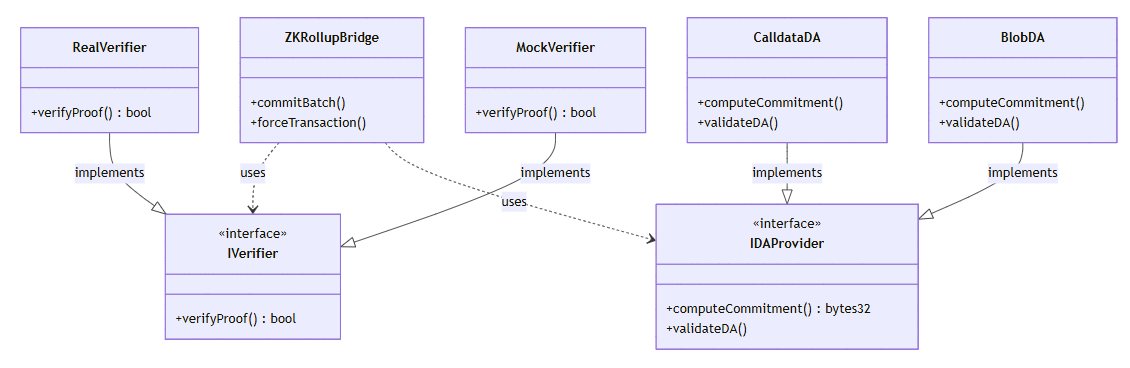
\includegraphics[width=0.95\linewidth]{figures/contract-interface.png}
  \caption{Contract Interface and Strategy Pattern.}
  \label{fig:contract-interface}
 \end{adjustwidth}
\end{figure}

\subsubsection{Architectural Components}

\subsubsubsection{ZKRollupBridge.sol}

\texttt{ZKRollupBridge.sol} is the primary entry point for settlement. It manages state root updates, validates submitted batch commitments, delegates proof verification to a verifier contract, and delegates DA validation to a DA provider contract.

A central design feature is the \textbf{Strategy Pattern} used to decouple the bridge from specific proof systems and DA mechanisms (Figure~\ref{fig:contract-interface}). The bridge maintains a mapping from \texttt{verifierId} to \texttt{IVerifier} implementations, allowing different verification behaviors to coexist under a unified interface. This makes it possible to use \texttt{verifierId=0} for real Groth16 verification on BN254, while reserving additional IDs for benchmarking-oriented verification paths for Plonky2 or Halo2.

\begin{lstlisting}[style=rustStyle, caption={Commit Batch with Modular Checks}, label={lst:commit-batch}]
function commitBatch(
    uint8 daId,
    uint8 verifierId,
    bytes calldata batchData,
    bytes calldata daMeta,
    bytes32 newRoot,
    bytes calldata proof
) external {
    _requireSequencer();

    // 1. Censorship Resistance Check
    if (forcedTxQueue.length > forcedHead) {
        // Ensure oldest forced tx hasn't expired
        // ...
    }

    // 2. Data Availability Validation
    IDAProvider provider = IDAProvider(daProviders[daId]);
    bytes32 daCommitment = provider.computeCommitment(batchData, daMeta);
    provider.validateDA(daCommitment, daMeta);

    // 3. ZK Proof Verification
    IVerifier selectedVerifier = verifiers[verifierId];
    // Construct public inputs: [oldRoot, newRoot, daCommitment_low, daCommitment_high]
    // Note: G2 points in proof must be swapped (imaginary, real) -> (real, imaginary)
    if (!selectedVerifier.verifyProof(..., inputs)) {
        revert InvalidProof();
    }

    // 4. Finalize State
    latestStateRoot = newRoot;
    emit BatchCommitted(..., newRoot);
}
\end{lstlisting}

\begin{itemize}
    \item \textbf{Modular Verification}: The bridge maps \texttt{verifierId} values to \texttt{IVerifier} implementations, enabling multiple proof systems to be selected without changing the bridge logic. In the current testbed, these verifiers are implemented as mock or stub contracts.
    \item \textbf{Split DA Commitment}: To satisfy typical scalar field constraints in public inputs, the 256-bit DA commitment (Keccak hash) is explicitly split into two 128-bit chunks (\texttt{daLow}, \texttt{daHigh}).
    \item \textbf{Access Control}: Governance-sensitive operations (e.g., updating sequencer address or registering new verifiers) are secured via \texttt{Ownable2Step}.
\end{itemize}

\subsubsubsection{Contract Storage Model}

The bridge maintains persistent state to track rollup progress and configuration.

\begin{figure}[htbp]
 \begin{adjustwidth}{0cm}{}
  \centering
  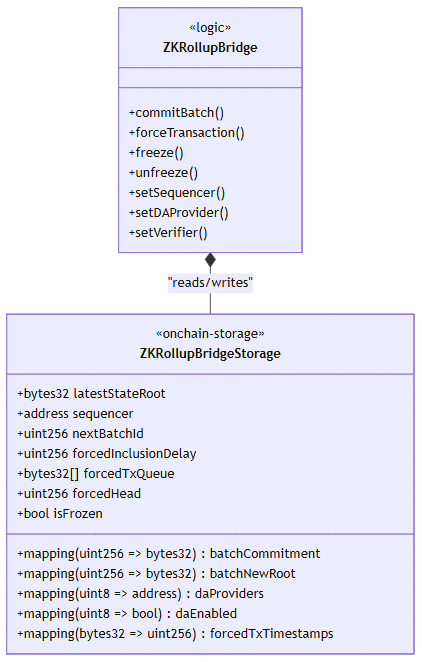
\includegraphics[width=0.95\linewidth]{figures/contract-storage-model.png}
  \caption{Contract Storage Model.}
  \label{fig:contract-storage}
 \end{adjustwidth}
\end{figure}

As illustrated in Figure~\ref{fig:contract-storage}, the storage layout includes the current \texttt{latestStateRoot}, batch commitment mappings, and configuration mappings for DA providers. This state is sufficient to support deterministic state progression and verifiable linkage between submitted batch commitments and the accepted rollup head.

\subsubsubsection{Censorship Resistance and Lifecycle}

The bridge incorporates a censorship-resistance mechanism that constrains sequencer behavior using an explicit lifecycle.

\begin{figure}[htbp]
 \begin{adjustwidth}{0cm}{}
  \centering
  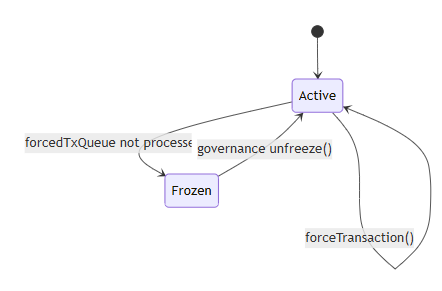
\includegraphics[width=0.95\linewidth]{figures/contact-state-daigram-lifecycle.png}
  \caption{Contract Lifecycle and Censorship Resistance.}
  \label{fig:contract-lifecycle}
 \end{adjustwidth}
\end{figure}

Through \texttt{forceTransaction}, users can enqueue transactions directly on L1. If the sequencer does not process forced transactions within \texttt{forcedInclusionDelay}, the bridge transitions from \textbf{Active} to \textbf{Frozen} (Figure~\ref{fig:contract-lifecycle}). In the Frozen state, normal batch commitments are halted, signaling that the centralized sequencer is not honoring the escape hatch guarantees. This mechanism protects users by preventing silent continuation under censorship assumptions and creates a clear safety boundary until governance action is taken or a mass-exit path (future work) is invoked.

\begin{lstlisting}[style=rustStyle, caption={Forced Transaction Mechanism}, label={lst:force-tx}]
function forceTransaction(bytes32 _txHash) external {
    if (isFrozen) revert BridgeFrozenError();

    // Set deadline for inclusion
    uint256 deadline = block.number + forcedInclusionDelay;
    forcedTxTimestamps[_txHash] = deadline;
    forcedTxQueue.push(_txHash);

    emit ForcedTransactionEnqueued(_txHash, deadline);
}
\end{lstlisting}

\subsubsubsection{DA Providers}

DA verification is abstracted behind the \texttt{IDAProvider} interface, enabling different validation logic depending on the chosen DA mode:

\begin{lstlisting}[style=rustStyle, caption={IDAProvider Interface}, label={lst:ida-provider}]
interface IDAProvider {
    function computeCommitment(
        bytes calldata batchData,
        bytes calldata daMeta
    ) external view returns (bytes32);

    function validateDA(bytes32 commitment, bytes calldata daMeta) external view;

    function mode() external pure returns (uint8);
}
\end{lstlisting}

\begin{itemize}
    \item \textbf{CalldataDA}: validates that the required batch data is present in the transaction payload.
    \item \textbf{BlobDA}: verifies \texttt{blobhash} against the expected commitment, ensuring the blob data matches the submission.
    \item \textbf{OffChainDA}: accepts a commitment (or pointer such as a CID) and delegates availability guarantees to an external data layer.
\end{itemize}

The \textbf{BlobDA} implementation (for EIP-4844) validates that the commitment matches the versioned hash of the attached blob, ensuring that the data is available on the consensus layer.

\begin{lstlisting}[style=rustStyle, caption={BlobDA Implementation}, label={lst:blob-da}]
contract BlobDA is IDAProvider {
    function validateDA(bytes32 commitment, bytes calldata daMeta) external view override {
        (bytes32 expectedVersionedHash, uint8 blobIndex) = abi.decode(daMeta, (bytes32, uint8));

        // 1. Check consistency
        if (commitment != expectedVersionedHash) revert InvalidCommitment();

        // 2. Verify against EVM intrinsic blobhash opcode
        bytes32 actual = blobhash(blobIndex);
        if (actual == bytes32(0)) revert NoBlobAttached();
        if (actual != expectedVersionedHash) revert BlobHashMismatch();
    }
}
\end{lstlisting}

\subsubsection{Verification Sequence}

\begin{figure}[htbp]
 \begin{adjustwidth}{0cm}{}
  \centering
  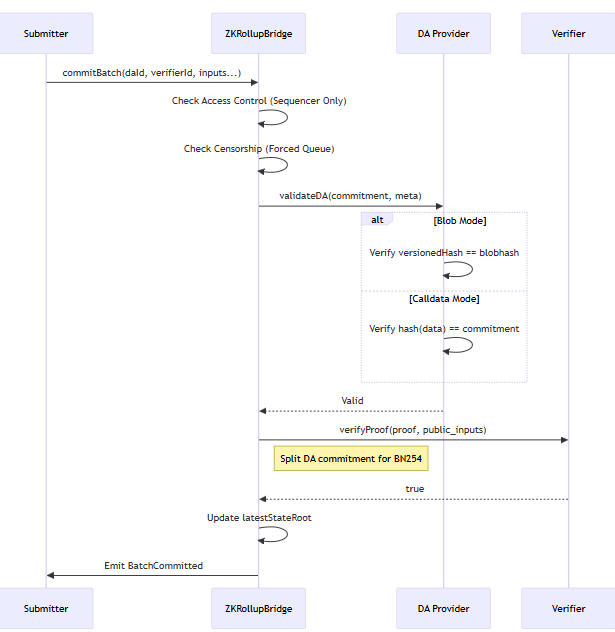
\includegraphics[width=0.95\linewidth]{figures/on-chain-verification-sequnce.png}
  \caption{On-Chain Verification Sequence.}
  \label{fig:contract-verification}
 \end{adjustwidth}
\end{figure}

When the Submitter calls \texttt{commitBatch}, the bridge executes a strict sequence of checks to ensure correctness and safety (Figure~\ref{fig:contract-verification}):
\begin{enumerate}
    \item \textbf{Access Control}: verifies that the caller is the authorized sequencer address.
    \item \textbf{Censorship Check}: verifies that forced transactions have not exceeded the allowed delay window.
    \item \textbf{DA Validation}: invokes the configured \texttt{IDAProvider} to validate the DA commitment (e.g., blobhash or calldata-derived hash).
    \item \textbf{Proof Verification}: invokes the selected \texttt{IVerifier} to verify the proof against public inputs (old root, new root, DA commitment chunks).
    \item \textbf{State Update}: updates \texttt{latestStateRoot} and emits \texttt{BatchCommitted} if all checks succeed.
\end{enumerate}

\subsubsection{Design Rationale and Trade-offs}

\paragraph{Modular Verification}
Decoupling the proof verification logic from the bridge (via the \texttt{IVerifier} interface) allows for upgrading the proof system without redeploying the main bridge contract. This is essential for a research testbed where cryptographic primitives are subject to change.

\paragraph{Censorship Resistance via Forced Transactions}
The \texttt{forceTransaction} mechanism (Listing~\ref{lst:force-tx}) introduces a trade-off: it adds complexity and potential state bloat (tracking the forced queue) but provides a fundamental security guarantee. Without it, the centralized sequencer could effectively freeze user funds. The use of a time-delayed trigger (\texttt{forcedInclusionDelay}) balances this by giving the sequencer a grace period to process legitimate transactions before the "freeze" mode is activated.

\paragraph{EIP-4844 Blob Integration}
Adopting EIP-4844 (Listing~\ref{lst:blob-da}) requires the contract to verify ephemeral data commitments (`blobhash`) rather than permanent calldata. This significantly reduces gas costs but requires the ecosystem (indexers, explorers) to support blob data retrieval, as it is pruned from L1 nodes after approx. 18 days.

\subsubsection{Current Limitations}

The current contract layer is fully functional for benchmarking and controlled experimentation, but it has known PoC limitations:
\begin{itemize}
    \item \textbf{Deposit Functionality}: \texttt{ZKRollupBridge.sol} does not currently implement a native \texttt{deposit} function for bridging assets from L1 to L2. Initial funding is handled via genesis allocation or sequencer-privileged minting in \texttt{dev\_mode}.
    \item \textbf{Proof Aggregation}: verification is executed per batch. Aggregating multiple batch proofs into a single L1 verification step—an important optimization for production cost reduction—is not yet implemented.
\end{itemize}



\subsection{Development Challenges and Solutions}

Throughout the prototype implementation, our team encountered three major technical challenges that significantly impacted development velocity and required systematic problem-solving approaches.

\textbf{1. Unfamiliarity with Rust Programming Language}

The team's primary experience with JavaScript, TypeScript, and Python created a steep learning curve when transitioning to Rust. Rust's unique ownership model, borrowing rules, and lifetime annotations—while providing memory safety guarantees—introduced conceptual barriers that were initially difficult to grasp. Simple operations straightforward in garbage-collected languages required careful consideration of ownership transfers, mutable versus immutable references, and lifetime bounds.

The compiler's strictness, though ultimately beneficial, initially resulted in prolonged development cycles as we struggled to satisfy the borrow checker. Common patterns such as sharing state across multiple components, implementing callbacks, or creating self-referential data structures proved particularly challenging. Error messages, while informative, required time to interpret correctly, especially for complex scenarios involving trait bounds and lifetime elision. Additionally, understanding the async/await ecosystem in Rust (\texttt{tokio}, futures, async traits) added another layer of complexity when implementing concurrent components like the L1 Event Listener and API handlers.

\textbf{2. Implementing Cryptographic Primitives and Zero-Knowledge Circuits}

The prover component, responsible for generating cryptographic validity proofs, presented the most technically demanding aspect of the project. Despite selecting Circom with Groth16 for its maturity and documentation (as outlined in Section 3.1.2), implementing the zero-knowledge circuits required deep understanding of finite field arithmetic, elliptic curve cryptography, and constraint systems.

Designing circuits to verify state transitions (OldRoot $\rightarrow$ NewRoot) for the Sparse Merkle Tree required translating high-level state update logic into arithmetic circuits with R1CS (Rank-1 Constraint System) constraints. This process was unintuitive and error-prone, as even simple operations like hash functions (Poseidon, SHA-256) required hundreds or thousands of constraints, impacting proof generation time. Debugging circuits proved particularly difficult since traditional debugging tools were inapplicable—identifying which constraint was violated and why required manual inspection and reasoning about the mathematical relationships.

Furthermore, integrating Circom circuits with our Rust codebase required FFI (Foreign Function Interface) bindings and careful management of witness generation, proving key paths, and proof serialization. The trusted setup ceremony for Groth16, though facilitated by existing tools, required understanding of the Powers of Tau and phase-2 ceremony processes. Performance optimization of the prover—crucial for achieving the throughput targets in our benchmarking experiments—demanded profiling constraint counts, exploring parallelization strategies, and tuning parameters like batch size to balance proving time against throughput.

\textbf{3. Component Integration and Inter-Process Communication}

While the modular architecture (Section 3.1.1) provided clear separation of concerns, integrating the Sequencer, Executor, Prover, Submitter, and on-chain contracts into a cohesive system presented significant coordination challenges. Each component, developed somewhat independently, needed to communicate reliably with precise data format agreements and error handling protocols.

Establishing efficient inter-process communication (IPC) mechanisms required architectural decisions about synchronous versus asynchronous patterns, message serialization formats (JSON, MessagePack, Protocol Buffers), and failure recovery strategies. The execution pipeline—Sequencer forwards sealed batches to Executor, which triggers Prover after state updates, and finally Submitter packages everything for L1 submission—required careful handling of failures at each stage. Any component crash or RPC error could lead to inconsistent states if not properly managed.

Synchronizing the Local State Cache in the Sequencer with the canonical Sparse Merkle Tree in the Executor proved particularly complex. State updates are asynchronous, and the Sequencer must handle scenarios where it continues accepting transactions based on slightly stale state while batches are being executed. Race conditions could occur if the Sequencer validated a transaction against state root $N$ while the Executor was processing batch $N+1$, potentially leading to nonce conflicts or double-spending attempts. Additionally, integrating with Ethereum testnets (Sepolia) introduced external dependencies on RPC endpoint reliability, gas price volatility, and transaction confirmation times, requiring robust retry logic and gas estimation strategies.

To address these challenges, we adopted a systematic, multi-faceted approach centered on iterative learning and pragmatic development practices.